%\documentclass[english,10pt]{article}
\documentclass[english,journal]{IEEEtran}
%\documentclass{report}
%\documentclass{acta}

\usepackage{cite}
\usepackage[pdftex]{graphicx}
\usepackage[cmex10]{amsmath}
\usepackage[tight,footnotesize]{subfigure}
\usepackage{fixltx2e}
\usepackage{url}
\usepackage{multirow}
\usepackage{latexsym}
\usepackage{amsfonts}
\usepackage{amssymb}
\usepackage{wasysym}
\usepackage{fancyhdr}
\usepackage{array}
\usepackage{longtable}
\usepackage{threeparttable}
\usepackage{acronym}
\usepackage{rotating}
\usepackage{rotate}
\usepackage{eurosym}
\usepackage[utf8]{inputenc}
\usepackage{color}
\usepackage{booktabs}
\usepackage{allrunes}
\usepackage{tabularx}
\usepackage{supertabular}
\usepackage{xcolor}
\usepackage{listings}
\usepackage{fancyvrb,relsize}
\usepackage{caption}
\usepackage{framed}
\usepackage{blindtext}
\usepackage{float}
\usepackage{epstopdf}
\usepackage{algpseudocode}
\usepackage{cprotect}
% always on last place
\usepackage{hyperref}

\DeclareGraphicsRule{.eps}{pdf}{.pdf}{`epstopdf #1}
\pdfcompresslevel=9

% hyperref options
\hypersetup{
    colorlinks,%
    citecolor=black,%
    filecolor=black,%
    linkcolor=black,%
    urlcolor=blue % yep, urls are blue and always will be...
}

% special environment for highlights, special concepts, etc.

% hyphenation style
\hyphenation{op-tical net-works semi-conduc-tor}

% new command for short vertical space
\newcommand{\vertbreak}{\vspace{1.75 mm}}

% new command for short vertical space
\newcommand{\shortvertbreak}{\vspace{1.50 mm}}

% new command for long vertical space
\newcommand{\longvertbreak}{\vspace{5.25 mm}}

% a thin space which allows line breaks
\newcommand*{\addthinspace}{\hskip0.08333em\relax}

% set caption font size to footnote size
\captionsetup{font={footnotesize}}

\makeatletter
\let\OldStatex\Statex
\renewcommand{\Statex}[1][3]{%
  \setlength\@tempdima{\algorithmicindent}%
  \OldStatex\hskip\dimexpr#1\@tempdima\relax}
\makeatother



\begin{document}

\title{A Model for Named Data Networking Inspired by 
Nonlinear Dynamical Systems}
\author{
    \IEEEauthorblockN{António D. N. Rodrigues}\\
    \IEEEauthorblockA{Faculdade de Engenharia da Universidade do Porto (FEUP), Porto, Portugal
    \\adamiaonr@fe.up.pt}
}

\maketitle

%%%%%%%%% ABSTRACT
\begin{abstract}

At the time of its inception, the Internet mostly served the purposes of 
communication between connected end-hosts. Now, at the World Wide Web 
era, the Internet is immersed in a content-centric paradigm, more 
concerned about content generation, sharing and access. Recently, 
a new research trend --- 
Information Centric Networking (ICN) --- started advocating for deep 
modifications on the Internet's network layer, making it content-centric by 
design, including the widespread use of in-network 
caching.\shortvertbreak

In this paper, we focus on the analysis of cache behavior in 
a specific ICN architecture --- Named 
Data Networking (NDN) --- under different caching policies, network 
topologies and content 
usage characteristics. To do so, we specify a simple and but modular NDN router 
model, loosely inspired in nonlinear dynamical 
systems. We implement the specified model in MATLAB, providing 
some simulation results with X simple caching policies, specifically (...).

\end{abstract}


%%%%%%%%% BODY TEXT

\section{Introduction}
\label{sec:intro}

Semi-supervised learning (SSL) is a branch of machine learning that makes use of 
unlabeled data in an attempt to improve the performance of purely supervised 
learning methods in cases where labeled data is `hard to get' and scarce, when compared to 
unlabeled data~\cite{chapelle2010semi,zhu05survey,zhu2009introduction}. Such scenarios are 
rather frequent, e.g. in application areas such as text classification, image 
recognition, web content analysis. Here we focus on 
the study of specific semi-supervised classification tasks, even though other 
sub-fields such as semi-supervised regression~\cite{chapelle2010semi} 
exist.\vertbreak

The work presented in this paper explores the field of semi-supervised learning, 
applied to a particular problem: text classification. We start by exploring 
a generative model for text classification --- Multinomial Naive Bayes (MNB)~\cite{McCallum98acomparison} --- still 
in its fully-supervised form. Based on that model, we then advance to a 
semi-supervised setting by combining it with the Expected Maximization (EM)~\cite{Nigam2000} 
algorithm, studying some techniques to augment it. We finally present results 
from our own and third-party implementations of such models, over the 
well-known 20 Newsgroups dataset~\cite{Lang95}.


\section{Named Data Networking (NDN)}
\label{sec:ndn}

In the Named Data Networking (NDN)~\cite{Jacobson2009} architecture, 
clients issue subscriptions for content 
objects by specifying 
a hierarchical (URL-like) content name, e.g. 
\verb+/pdeec+\addthinspace\verb+/mtsp/+\addthinspace\verb+2014/+, which is 
directly used in NDN packets. 
Destination network locators (e.g. IP addresses) are not used in this case, as 
NDN routers are able 
to forward such packets towards appropriate content-holding destinations, solely based 
on such names. NDN contemplates two fundamental types of packets, `Interest' and `Data' packets, 
used for content subscriptions and publications, respectively. Interest packets 
are originally released into the network by clients willing to access a 
particular content, addressing it via its content name, while Data packets 
carry the content itself.\shortvertbreak

\begin{figure}[h!]

    \centering
    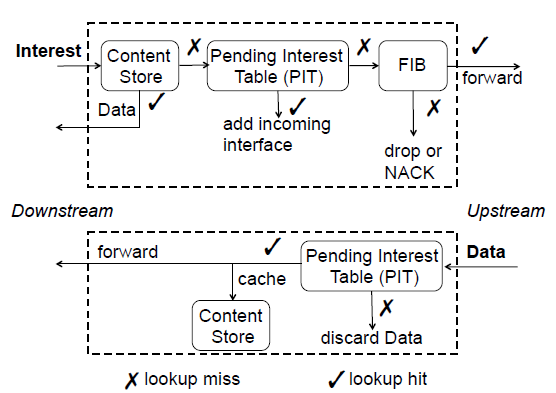
\includegraphics[width=0.35\textwidth]{figures/ndn-forwarding-engine.png}
    \cprotect\caption{Interest and Data packet processing according to NDN's 
        forwarding engine~\cite{Yi2012}.}
    \label{fig:ccn-icn-ndn-forwarding-engine}

\end{figure}

An NDN router is conceptually composed by three main elements: (1) a 
Forward Information 
Base (FIB), (2) a Pending Interest Table (PIT) and (3) a Content Store 
(CS)~\cite{Jacobson2009}:

\begin{itemize}

    \item \textbf{Forward Information Base (FIB):} Routing\slash forwarding 
        table holding entries 
        which relate a name prefix and a list of router interfaces to which 
        Interest packets matching that content name prefix should be forwarded 
        to.
    \item \textbf{Pending Interest Table (PIT):} A table which keeps track of 
        the mapping between arriving Interest packets and 
        the interfaces these have been received from, in order to save a reverse 
        path for Data packets 
        towards one or more subscribers (this may be a 1:N mapping, as an 
        Interest packet matching the same content may be received in 
        multiple interfaces).
    \item \textbf{Content Store (CS):} A cache for content, indexed by content 
        name or item. This novel element allows for content storage at the 
        network level. In-network caching allows an Interest to be satisfied 
        by a matching Data packet in any location other than the original 
        producer of the content, constituting one of the main 
        content-oriented characteristics of NDN.

\end{itemize}

In NDN, communication is receiver-driven, i.e. having the desire to fetch 
a particular content, a client releases an Interest packet into the network 
so that it is forwarded towards an appropriate content holder. In 
Figure~\ref{fig:ccn-icn-ndn-forwarding-engine}~\cite{Yi2012}, we provide a 
graphical description 
of the mechanics of the forwarding engine of an NDN router, supported by 
the textual description provided below:

\begin{enumerate}

    \item An Interest packet arrives on an interface (e.g. \verb+iface0+) of an NDN router.
    \item A longest prefix match on the content name specified in the Interest (e.g. \verb+name+) 
        is performed. The NDN router will now look in its CS, PIT and FIB, in 
        that order, in order to resume the forwarding action:
        \begin{enumerate}

            \item If there's a match in the router's CS, a copy of the respective 
                CS entry will be sent back via \verb+iface0+, the Interest 
                packet is dropped. Depending on the pre-specified 
                caching policy (e.g. MRU, LRU, LFU~\footnote{\url{http://en.wikipedia.org/wiki/Cache_algorithms}}, 
                etc.), the organization of the CS 
                may change at this point. \textbf{End.}

            \item Else if there is an (exact) match in the PIT, \verb+iface0+ is 
                added to the mapping list on the respective entry. The 
                Interest packet is dropped (as a previous one has already been 
                sent upstream). \textbf{End.}

            \item Else if only a matching FIB entry is found, the Interest 
                packet is forwarded upstream, via all remaining interfaces on the 
                list (except \verb+iface0+), towards an eventual content holder. A PIT 
                entry $<$\verb+name+, \verb+iface0+$>$ is added. \textbf{End.}

            \item Else if there is no match at all, the Interest packet is 
                simply discarded. \textbf{End.}\shortvertbreak

        \end{enumerate}

\end{enumerate}

Note that in NDN only Interest packets are forwarded: intermediate NDN 
routers (i.e. between client and content holder) forward the 
Interests and have their respective PIT tables updated with Interest-to-interface 
mappings, pre-establishing a reverse path for Data packets to follow as soon as a 
content holder is found. When the reverse path is `followed' (i.e. in the 
`downstream' direction, lower part of Figure~\ref{fig:ccn-icn-ndn-forwarding-engine}), each 
intermediate NDN router receiving a 
Data packet looks in its PIT for $<$\verb+name+, \verb+iface+$>$ entries, 
and forwards the Data packet through all matching interfaces. In addition, a 
CS entry is created to cache the content locally at the router (again, depending 
on the caching policy, the organization of the CS may change at this point). If a Data packet 
with no matching PIT entries arrives, it is treated as unsolicited and discarded.



\section{Methodology}
\label{sec:methodology}

In this section we describe the proposed NDN model in detail. We start with 
an overview, setting the notation and crudely establishing its relation 
with nonlinear dynamical systems. We then continue with a detailed description 
of each model component and related procedures.

\subsection{Overview}
\label{subsec:meth-overview}

We consider a conceptual NDN network composed by three main types of 
entities: (1) 
$|R|$ NDN routers\footnote{Here we use the notation $|E|$ to 
represent the number of elements of type $E$.} $R_r$, $r = \{1,2,...,|R|\}$, 
organized in some type of topology (e.g. cascade, tree, etc.); (2) a set of 
$|C|$ clients $C_c$, $c = \{1,2,...,|C|\}$; and a single 
content server $S$, holding $|O|$ different content objects $O_o$, 
$o = \{1,2,...,|O|\}$ (e.g. $|O|$ different photos).\shortvertbreak

Clients issue requests for content objects $O_o$, i.e. Interest packets $i_{O_o}$, which 
are propagated through NDN routers towards the content server $S$, and 
eventually followed by Data packets 
$d_{O_o}$, containing the requested content object. We represent the 
elementary set of signals fed to\slash read from the inputs\slash outputs of the 
aforementioned basic 
entities, at some discrete time $n$, as a $2\,|O| \times 1 $ vector in the form

\begin{equation}
    \textbf{v}[n] = \begin{bmatrix}  i_{O_1}         \\ 
                            i_{O_2}         \\ 
                             ...            \\ 
                            i_{O_{|O|}}     \\ 
                            d_{O_1}         \\ 
                            d_{O_2}         \\ 
                             ...            \\ 
                            d_{O_{|O|}}     \\ \end{bmatrix}
    \label{eq:signal}
\end{equation}\shortvertbreak

Each component $i_{O_o}$ or $d_{O_o}$ may assume an integer value, i.e. $i_{O_o}, d_{O_o} \in \mathbb{N}_0 = \{0, 1, 2, ... \}$, 
representing the absence (in case of $i_{O_o}, d_{O_o} = 0$) or presence (in case of $i_{O_o}, d_{O_o} > 0$) of an 
Interest\slash Data packet, at a given discrete time $n$. E.g. considering a setting 
with $|O| = 2$ content objects, a value of \textbf{x} corresponding to the presence 
of two Interests for content $O_1$ and one Data packet for $O_2$ (with the absence 
for the remaining components) would be encoded as

\begin{equation}
    \textbf{v}[n] = \begin{bmatrix}     2   \\ 
                                        0   \\ 
                                        0   \\ 
                                        1   \\ \end{bmatrix}
    \label{eq:signal-eg}
\end{equation}\shortvertbreak

With this 
representation, we capture situations in which a network 
entity may simultaneously receive\slash issue any Interest or Data packet at 
its input\slash output. Our models for NDN routers, clients or servers can be 
seen as nonlinear dynamical subsystems, accepting inputs \textbf{u} and producing 
outputs \textbf{y}, in the form shown in eq.~\ref{eq:signal} 
and eq.~\ref{eq:signal-eg}. Furthermore, each one of these subsystems exhibits one or 
more types of state \textbf{x} (e.g. the composition of a Content Store or a Pending 
Interest Table), which evolves according to nonlinear dynamics $\mathcal{H}$, 
driven by \textbf{u} and the current state \textbf{x}:

\begin{equation}
    \textbf{x}[n + 1] = \mathcal{H}(\textbf{x}[n],\textbf{u}[n])
    \label{eq:state}
\end{equation}%\shortvertbreak

Outputs \textbf{y} are nonlinearly related to some current state \textbf{x} and input \textbf{u}:

\begin{equation}
    \textbf{y}[n] = \mathcal{G}(\textbf{x}[n],\textbf{u}[n])
    \label{eq:outputs}
\end{equation}%\shortvertbreak

We also note that in some subsystems, namely at the clients $C$, the outputs 
\textbf{y} may include a stochastic component $w$ (e.g. in cases where Interest 
signals are randomly generated):

\begin{equation}
    \textbf{y}[n] = \mathcal{G}(\textbf{x}[n],\textbf{u}[n]) + w
    \label{eq:clients}
\end{equation}%\shortvertbreak

In the next subsections, we describe each one of the nonlinear subsystems in 
detail, including the types of state and associated nonlinear dynamics.

\subsection{NDN Router Model}
\label{subsec:meth-overview}

An NDN router is the central entity of the presented model, acting 
as the main agent of NDN's forwarding engine. It is also the more complex entity, 
including a set of submodules, already 
mentioned in Section~\ref{sec:ndn}: (1) the Pending Interest Table (PIT); (2) 
the Content Store (CS); and (3) the Forward Information Base (FIB). We first 
provide an overview of our NDN router module, and then proceed with the description 
of each one of its submodules.\shortvertbreak

\begin{figure}[h!]

    \centering
    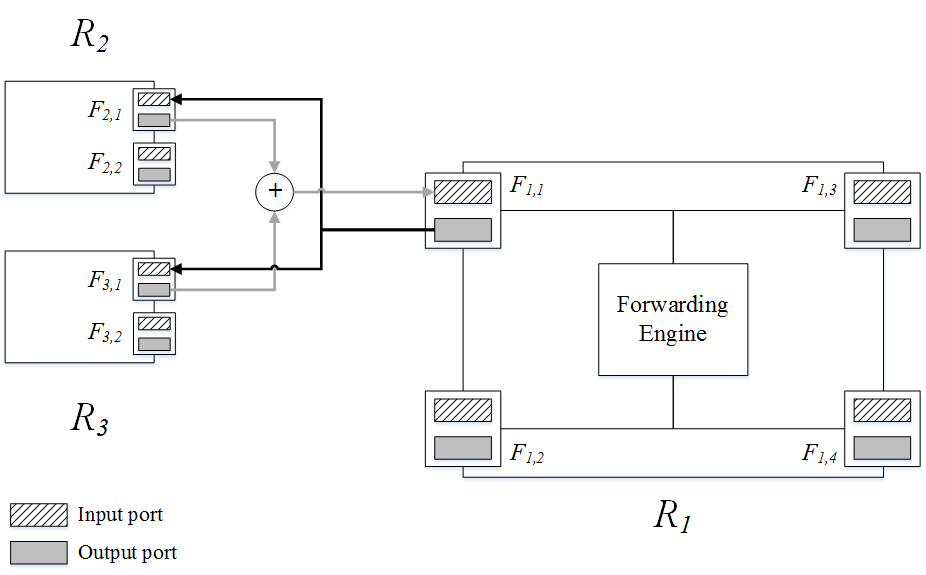
\includegraphics[width=0.40\textwidth]{figures/ndn-router-overview.png}
    \cprotect\caption{Graphical depiction of our NDN router model.}
    \label{fig:ndn-router-overview}

\end{figure}

Figure~\ref{fig:ndn-router-overview} provides a graphical description of the proposed 
router model. A router $R$ contains a set of $|F|$ interfaces $F$, used to interconnect 
it to other entities (e.g. some other router $R'$, a client $C$ or a server 
$S$). Each interface can subsequently be divided into one input and one output 
port, which `cross-connect' with the ports of the attached 
interfaces (see Figure~\ref{fig:ndn-router-overview}). We use the notation 
$F_{r,f,in}$ or $F_{r,f,out}$, to refer to the 
input\slash output ports of an interface with index $f$, of a router $R_r$\footnote{We 
adopt a flexible notation, sometimes referring to an interface as 
$F_{r,f}$ when there is no need to specify a particular port.}.\shortvertbreak

Taking Figure~\ref{fig:ndn-router-overview} as a supporting example, the act of 
forwarding some set of Interest\slash Data packets from a router $R_1$, 
over some interface $F_1$, is modeled by having $R_1$ fill $F_{1,1,out}$ with 
some set of signals \textbf{y}, following the encoding shown in 
Section~\ref{subsec:meth-overview}. Conversely, the act of receiving some set 
of Interest\slash Data packets is modeled by having routers $R_2$ and $R_3$ --- 
connected with $F_{1,1}$ via $F_{2,1}$ and $F_{3,1}$ --- fill $F_{2,1,in}$ and $F_{3,1,in}$ 
with \textbf{u} \footnote{In fact, this procedure can be extended to any network entity, let 
it be a router, a client or a server.}. As seen in Figure~\ref{fig:ndn-router-overview}, 
more than one entity may be connected to some interface, in which case the 
signals \textbf{y} originating from the interconnected interfaces' output ports, 
e.g. $F_{2,1,out}$ and $F_{3,1,out}$, are combined and summed at the other 
end's input port, e.g. $F_{1,1,in}$. While the use of interfaces and 
input\slash output ports may be seen as a case of over engineering, we argue 
it makes our model robust, highly modular and capable of supporting multiple 
network topologies.\shortvertbreak

\subsubsection{Pending Interest Table (PIT)}
\label{subsec:meth-pit}

In the same way that the FIB commands the forwarding of Interests, the PIT 
commands the forwarding of Data packets. The composition of the 
PIT is more dynamic than that of the FIB, being dependent on the flow of 
Interest and Data signals through the NDN router. We model the PIT as a 
$|O| \times |F|$ matrix in the form:

\begin{equation}
\textbf{PIT} = \begin{bmatrix} 1 & 0 & 0 & 0  \\ 
                1 & 0 & 0 & 0               \\ 
                0 & 1 & 0 & 0               \\ 
                0 & 1 & 0 & 0               \\ \end{bmatrix}
    \label{eq:pit}
\end{equation}\shortvertbreak

\textbf{PIT}\footnote{We use the form `PIT' for general references to the Pending 
Interest Table, and `\textbf{PIT}' when referring to its matrix form, as in eq.~\ref{eq:pit}. 
This dual representation is extended to the FIB and CS.} entries 
$(o,f)$ are encoded as 0 or 1: if $(o,f) = 1$, Interests for content object 
$O_o$ have been previously received in interface $F_{r,f}$, and so Data 
packets $d_{O_o}$ shall be forwarded via $F_{r,f}$; on the other hand, 
if $(o,f) = 0$, $d_{O_o}$ should not be forwarded via that 
interface. The arrival of Interest and Data packets influences the composition of 
the PIT over time, each triggering special routines --- \textbf{PIT::updateOnInterest()} and 
\textbf{PIT::updateOnData()} --- shown below. We consider 
special $2\,|O| \times |F|$ matrices \textbf{U} and \textbf{Y}, corresponding to the concatenation of 
all the column vectors $\textbf{u}_{r,f}$ and $\textbf{y}_{r,f}$, i.e. the contents from the input and output ports 
of all the interfaces $F_{r,f}$, at some router $R_r$:

\begin{equation}
\textbf{U} = \begin{bmatrix} \textbf{u}_{r,1} & \textbf{u}_{r,2} & ... & \textbf{u}_{r,|F|} \end{bmatrix}
    \label{eq:a}
%\end{equation}\shortvertbreak
\end{equation}

\begin{equation}
\textbf{Y} = \begin{bmatrix} \textbf{y}_{r,1} & \textbf{y}_{r,2} & ... & \textbf{y}_{r,|F|} \end{bmatrix}
    \label{eq:b}
%\end{equation}\shortvertbreak
\end{equation}\shortvertbreak

\begin{algorithmic}[1]

\State \textbf{define} PIT::updateOnInterest(\textbf{U}):
\State
    \State $\textbf{U}' \leftarrow \textbf{U}(1:|O|,:)$
%    \State $\textbf{D} \leftarrow$ diag$(\neg(\textbf{PIT} \times \textbf{1}))$
    \State $\textbf{Y}'_i \leftarrow$ $\neg(\textbf{PIT} \times \textbf{1}^{|F|}) \ \& \ (\textbf{U}' \times \textbf{1}^{|F|})$
%    \State $\textbf{B} \leftarrow \textbf{D} \times \textbf{U}'$ 
    \State $\textbf{Y}'_i \leftarrow \textbf{FIB} \ \& \ (\textbf{Y}'_i \times {\textbf{1}^{|F|}}^{T})$
    \State $\textbf{Y}_i \leftarrow \begin{bmatrix} \textbf{Y}'_i \\ \textbf{0}^{|O| \times |F|} \end{bmatrix}$
    \State \textbf{PIT} $\leftarrow$ \textbf{PIT} $|$ $\textbf{U}'$ 
    \State \Return $\textbf{Y}_i$

\end{algorithmic}\shortvertbreak

Upon the reception of Interest signals, i.e. $\textbf{U}'$ (the first $|O|$ rows 
of $\textbf{U}$), we first identify the content items $O_o$, or the row indexes $o$ of the 
\textbf{PIT}, for which there are \textbf{no} pending Interests (line 4). For 
convenience, we often recur to binary operations (negation `$\neg$', 
conjunction `$\&$', disjunction `$|$') over matrices: e.g. in line 4, after 
summing all columns of the \textbf{PIT}\footnote{We use the notation $\textbf{1}^{m}$ for the $m \times 1$
sum vector, i.e. $\textbf{1}^{m} = [1\,1\,...\,1]^{T}$, and $\textbf{1}^{m \times n}$ for an $m \times n$ 
matrix solely composed by '1'. Equivalently, we also use $\textbf{0}^{m}$ and $\textbf{0}^{m \times n}$.}, we negate the 
result, obtaining a binary encoded $|O| \times 1$ 
column vector which indicates the absence (encoded as  `1') and presence 
(encoded as `0') of pending Interests for some content object $O_o$. Still in 
line 4, we obtain a $|O| \times 1$ column vector, $\textbf{Y}'_i$, which encodes 
Interest signals which are not already stored in the PIT, and that the NDN router needs to forward upstream. This is 
accomplished by taking the logic AND, `$\&$', between $\neg(\textbf{PIT} \times \textbf{1}^{|F|})$ and 
$\textbf{U}'$. Note that even 
if $\textbf{U}'$ includes some $i_{O_o} > 1$, we only need to forward one Interest 
over the interfaces specified in the FIB, and so the binary encoding of $\textbf{Y}'_i$, 
resulting from the use of binary operations, neatly serves our purposes. The operation 
in line 5 results in a final form of $\textbf{Y}'_i$, which assigns the 
Interest signals to be forwarded upstream to the appropriate interfaces, according to the FIB. 
In line 6 we finally obtain $\textbf{Y}_i$, a $2\,|O| \times |F|$ matrix compliant 
with the format shown in eq.~\ref{eq:b}. 
In line 7, the 
contents of the \textbf{PIT} are updated by performing a logic OR, `$|$', with $\textbf{U}'$, so 
that it registers all the newly received 
Interest signals and their correspondence to interfaces. This last step is important, 
as it allows future Data packets to be forwarded downstream over the requesting 
interfaces.\shortvertbreak

\begin{algorithmic}[1]

\State \textbf{define} PIT::updateOnData($\textbf{U}$):
\State
    \State $\textbf{U}' \leftarrow \textbf{U}(|O|+1:2\,|O|,:)$
    \State $\textbf{G} \leftarrow (\textbf{U}' \times \textbf{1}^{|F|}) \times {\textbf{1}^{|F|}}^{T}$
%    \State $\textbf{D} \leftarrow \textbf{U}' \times \textbf{1}$
    \State $\textbf{Y}'_d \leftarrow$ $\textbf{PIT} \ \& \ \textbf{G}$
    \State $\textbf{Y}_d \leftarrow$ $\begin{bmatrix} \textbf{0}^{|O| \times |F|} \\ \textbf{Y}'_d \end{bmatrix}$
    \State \textbf{PIT} $\leftarrow$ $\textbf{PIT} \ \& \ \neg\textbf{G}$ 
    \State \Return $\textbf{Y}_d$

\end{algorithmic}\shortvertbreak

%With the explanation given above for the \textbf{PIT::updateOnInterest()} routine, 
%the understanding of \textbf{PIT::updateOnData()} is left to the reader. 
Note that 
the objective of PIT::updateOnData() is the reverse operation of PIT::updateOnInterest(), i.e. forwarding Data 
packets over the interfaces for which there is a registered Interest in the \textbf{PIT}, with 
the result encoded in matrix $\textbf{Y}_d$. $\textbf{G}$ consists in a $|O| \times |F|$ matrix, which expands the single-column 
vector $\textbf{U}' \times \textbf{1}^{|F|}$ to $|F|$ columns (line 4), making it ready 
for the subsequent AND (`\&') operations (lines 5 and 7). The final 
step of the operation (line 7) consists in erasing 
all Interest registrations which have been successfully attended.\shortvertbreak

As a final remark, we can now identify the \textbf{PIT} as one form of state 
\textbf{x}, which is driven by the nonlinear dynamics specified on the 
PIT::updateOnInterest() and PIT::updateOnData() routines (line 7, in both cases). 
Furthermore, both routines also contribute to the generation of outputs, 
in the form of matrices $\textbf{Y}_i$ and $\textbf{Y}_d$.\shortvertbreak

\subsubsection{Content Store (CS)}
\label{subsec:meth-cs}

We model the Content Store (CS), i.e. the NDN router's cache, as an $|O| 
\times |P|$ matrix, in which $|P|$ is the size of the CS, i.e. maximum 
number of content objects it is able to accommodate at any given point in time. 
We use $P$ to represent a position or slot in the CS, which is able to hold a single 
content object $O_o$ (here we do not consider a notion of content object size, 
an object always fits in a slot $P$). E.g. in eq.~\ref{eq:cs} we show the encoding 
of the \textbf{CS} for $R_1$ in Figure~\ref{fig:fib-topo}, with $|P| = 2$, 
which is shown to contain content objects $O_2$ and $O_4$\footnote{Usually, 
we consider $|P| << |O|$.}.

\begin{equation}
\textbf{CS} = \begin{bmatrix} 0 & 0             \\ 
                1 & 0                           \\ 
                0 & 1                           \\ 
                0 & 0                           \\ \end{bmatrix}
    \label{eq:cs}
\end{equation}\shortvertbreak

Again, we follow a binary encoding, using $(o, p) = 1$ to indicate the 
presence of content $O_o$ at slot $P_p$, and $(o, p) = 0$ as an indication of 
its absence. Each slot is assigned a different integer 
index, i.e. $P_p$, with $p = \{1, 2, ..., |P|\}$, which express the idea of `cache levels': 
$O_o$, occupying slot $P_2$, is at the 2\textsuperscript{nd} 
(highest) position of the \textbf{CS}. $P_1$ is usually interpreted as the `highest' 
level, and $P_{|P|}$ the `lowest', nevertheless the meaning is of the `levels' 
is often dependent on the cache algorithm implemented by the CS.\shortvertbreak
%In fact, we 
%model a CS as having a general behavior (presented in this section), and a specific 
%behavior, which depends on the cache algorithm the CS implements. We discuss cache 
%algorithms in Section~\ref{subsec:meth-caching-algs}.\shortvertbreak

Note that \textbf{CS} must obey a set of constraints, since (1) 
each slot can only hold a single content object, and (2) it is inefficient for 
the \textbf{CS} to hold multiple copies of a content $O_o$. Specifically, the 
conditions for the validity of \textbf{CS} are:

\begin{equation}
    \sum_{o=1}^{|O|} \textbf{CS}_{o,p} \le 1 \quad \forall \ p \in {1, 2, ..., |P|}
    \label{eq:cs-constraints-1}
\end{equation}

\begin{equation}
    \sum_{p=1}^{|P|} \textbf{CS}_{o,p} \le 1 \quad \forall \ o \in {1, 2, ..., |O|}
    \label{eq:cs-constraints-2}
\end{equation}

Similarly to the PIT, the operations related to the CS are implemented by two 
routines: \textbf{CS::updateOnInterest()} and \textbf{CS::updateOnData()}. While 
the behavior of CS::updateOnData() is specific to a particular cache 
algorithm (see Section~\ref{subsec:meth-caching-algs}), that of CS::updateOnInterest() 
is rather general, consisting in the generation of a pair of $|O| \times |F|$ 
matrices, $[\textbf{Y}_h, \textbf{R}]$. In short, $\textbf{Y}_h$ encodes 
the Data packets for which there are cache hits, already assigned to the 
appropriate interface columns; and $\textbf{R}$ encodes all the Interest signals 
for which there were no cache hits\footnote{Due to space constraints, we do not 
show the algorithm of CS::updateOnInterest(), which can nevertheless be 
consulted in \url{github.com/adamiaonr/mtsp-project}.}.\shortvertbreak

Again, \textbf{CS} may be seen as the other form of state in the NDN router 
subsystem, driven by the nonlinear dynamics specified by each different 
cache algorithm. Furthermore, the CS::updateOnInterest() 
routine, common to all caching policies, contributes to the generation of the 
output matrix \textbf{Y} via $\textbf{Y}_h$.\shortvertbreak

\subsubsection{Forwarding Information Base (FIB)}
\label{subsec:meth-fib}

The FIB is important for the act of forwarding Interest packets towards 
appropriate content sources, by indicating the interfaces $F$ over which such 
sources are reachable. For each NDN router $R$, we model the FIB as a simple 
$|O| \times |F|$ matrix in the form

\begin{equation}
\textbf{FIB} = \begin{bmatrix} 1 & 0 & 0 & 0  \\ 
                1 & 0 & 0 & 0               \\ 
                0 & 1 & 0 & 0               \\ 
                0 & 1 & 0 & 0               \\ \end{bmatrix}
    \label{eq:fib}
\end{equation}\shortvertbreak

The \textbf{FIB} encoding shown in eq.~\ref{eq:fib} would be held by router $R_1$ in the 
simple topology shown in Figure~\ref{fig:fib-topo}. \textbf{FIB} entries 
$(o,f)$ are encoded as 0 or 1: if $(o,f) = 1$, content objects of 
type $O_o$ are accessible via interface $F_f$, meaning that Interests 
$i_{O_o}$ shall be forwarded via $F_f$; on the other hand, 
if $(o,f) = 0$, $i_{O_o}$ should not be forwarded via that interface. 
Following the same type of operations described for the PIT 
in Section~\ref{subsec:meth-pit}, we now present the algorithm followed by NDN 
routers to forward Interest signals, which uses PIT::updateOnInterest() as well 
as CS::updateOnInterest():\shortvertbreak 

\begin{algorithmic}[1]

\State \textbf{define} Router::forward($\textbf{U}$):
\State
    \State $[\textbf{Y}_h, \textbf{R}] \leftarrow \text{CS::updateOnInterest(\textbf{U})}$
    \State $\textbf{Y}_i \leftarrow \text{PIT::updateOnInterest(\textbf{R})}$
%    \State $\textbf{B}' \leftarrow \textbf{B} \times \textbf{1}$
%    \State $\textbf{L} \leftarrow$ diag$(\textbf{B}) \times$ \textbf{FIB}
    \State $\textbf{Y}_d \leftarrow \text{PIT::updateOnData(\textbf{U})}$
    \State $F_{n,1:|F|,out} \leftarrow (\textbf{Y}_i + \textbf{Y}_h + \textbf{Y}_d)$

\end{algorithmic}\shortvertbreak

From CS::updateOnInterest(), we obtain $\textbf{Y}_h$, the output Data signals 
resulting from cache hits, and \textbf{R}, the Interest signals for which 
there were no cache hits. We use \textbf{R} as an input to PIT::updateOnInterest(), 
ultimately obtaining $\textbf{Y}_i$, the output Interest signals. Finally, 
the router processes the Data input signals on \textbf{U}, generating the 
Data output signals, $\textbf{Y}_d$, according to the behavior of 
PIT::updateOnData(). The last 
operation (line 6) refers to 
the (parallelized) `filling' of the output ports of all the interfaces $F$ of router $R_r$, 
with both $\textbf{Y}_i$, $\textbf{Y}_h$ and $\textbf{Y}_d$, which together 
consist in the complete output matrix \textbf{Y}.\shortvertbreak

In our model, the composition of the \textbf{FIB} is established at an initial phase, 
not suffering any further alterations (more details in 
Section~\ref{subsec:meth-conn-dots}). Note 
that the FIB only commands Interest forwarding actions, not participating in the 
forwarding of Data packets.

\begin{figure}[h!]

    \centering
    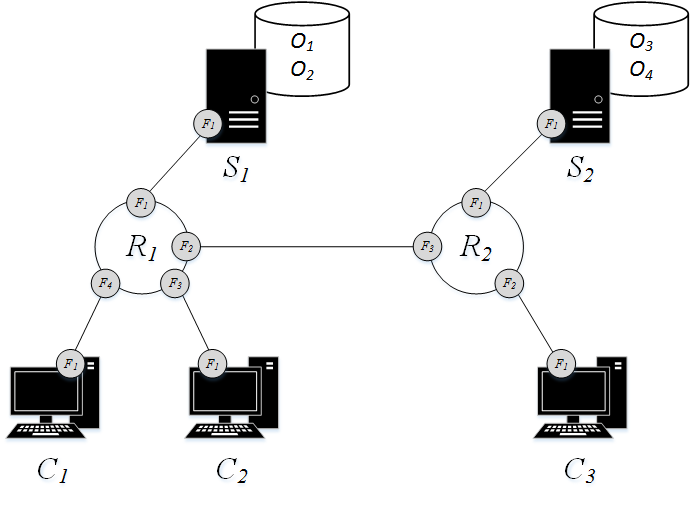
\includegraphics[width=0.30\textwidth]{figures/fib-topo.png}
    \cprotect\caption{Simple example of an NDN network topology.}
    \label{fig:fib-topo}

\end{figure}

\subsection{Endpoints}
\label{subsec:meth-endpoints}

In our model we consider two forms of endpoints: clients $C$ and servers $S$. 
Clients generate Interests for content, i.e. vectors in the form of \textbf{v} 
in eq.~\ref{eq:signal}, while servers hold caches in which content objects persist 
and are always available.\shortvertbreak

The operation of servers is simple, basically consisting in mirroring the 
Interest signals received as input, according to the contents of their 
persistent CS:\shortvertbreak

\begin{algorithmic}[1]

\State \textbf{define} Server::mirror(\textbf{U}):
\State
    \State $\textbf{U}' \leftarrow \textbf{CS} \ \& \ \textbf{U}$ 
    \State
    \State $\textbf{Y}_h \leftarrow \begin{bmatrix} \textbf{0}^{|O| \times |F|} \\ \textbf{U}'(1:|O|,:) \end{bmatrix}$ 
    \State $F_{n,1:|F|,out} \leftarrow \textbf{Y}_h$

\end{algorithmic}\shortvertbreak

Clients generate Interest signals according 
to some popularity distribution such as Zipf~\cite{6038471}. In our model, each 
client $C$ independently takes a $|O| \times 1$ vector $\textbf{q}$, containing 
the Interest generation probabilities for each content object $O_o$, $q_o$. During 
a simulation, at 
some discrete time instant $n$, a client $C$ generates an Interest for content 
object $O_o$ with probability $q_o$.

\subsection{Cache Algorithms}
\label{subsec:meth-caching-algs}

In order to evaluate the feasibility of the proposed model, we consider two 
well known cache algorithms, LRU~\cite{Johnson:1994:LOH:645920.672996} and 
MRU~\cite{Chou:1985:EBM:1286760.1286772}, in addition to a Random caching policy, 
which randomly evicts a content object cached at the CS, in the presence 
of a new object to be cached. In practice, each different caching 
algorithm constitutes a different implementation of the CS::updateOnData() 
routine, mentioned in Section~\ref{subsec:meth-cs}, and basically defines 
the `type' of CS for an NDN router as an input parameter.\shortvertbreak

As the design of cache replacement policies has not been the 
main purpose of this work, we do not explain the aforementioned algorithms in 
detail. Their implementation has nevertheless been part of this work, and can 
be consulted in~\url{github.com/adamiaonr/mtsp-project}.

\subsection{Network Topologies}
\label{subsec:meth-topologies}

We represent a network topology using a square matrix \textbf{T}, 
with dimension $|R|+|C|+|S|$. For representation purposes, we attribute an 
integer index to each one of the network nodes, and so each elements $(i,j)$ of the 
matrix corresponds to interconnections between network entities with indexes $i$ and $j$. The 
values at each $(i,j)$ position identify the \textbf{near end interface} of the 
connection, i.e. the interface at entity $i$. E.g. the matrix \textbf{T} shown 
in eq.~\ref{eq:topo} encodes the topology shown in Figure~\ref{fig:fib-topo}. In this case, 
we attribute the integers 1 to 7 to the network entities, starting with the 
clients $C_1$ to $C_3$, then routers $R_1$ and $R_2$ and 
finally the servers $S_1$ and $S_2$.

\begin{equation}
\textbf{T} = \begin{bmatrix} 
                0 & 0 & 0 & 1 & 0 & 0 & 0               \\ 
                0 & 0 & 0 & 1 & 0 & 0 & 0               \\ 
                0 & 0 & 0 & 0 & 1 & 0 & 0               \\ 
                4 & 3 & 0 & 0 & 2 & 1 & 0               \\ 
                0 & 0 & 2 & 3 & 0 & 0 & 1               \\ 
                0 & 0 & 0 & 1 & 0 & 0 & 0               \\ 
                0 & 0 & 0 & 0 & 1 & 0 & 0               \\ \end{bmatrix}
    \label{eq:topo}
\end{equation}

\subsection{`Connecting the Dots'}
\label{subsec:meth-conn-dots}

Given all the `pieces of the puzzle', we can now describe how the proposed model 
behaves under simulation. A simulation is composed by two distinct phases: (1) 
a setup phase, and (2) a round phase. During phase 1, the simulation engine 
interprets (a) the topology matrix $\textbf{T}$, (b) the content parameters (number of 
contents $|O|$ and popularity distribution $\textbf{q}$) and (c) the CS parameters 
(size $|P|$ and type), creating the overall network entities --- routers, clients and 
servers --- as well as the appropriate interconnections.\shortvertbreak

In phase 2, given a number of rounds $|N|$, the simulation engine iteratively 
executes the following algorithm:\shortvertbreak

\begin{algorithmic}[1]

\State \textbf{define} SimEngine::run():
\State

    \For{ ($N \leftarrow 1$; $N < |N|$; $N$++)} 

        \ForAll{$C_c$}
            \State $C_c$.requestContent()
        \EndFor
        \ForAll{$R_r$}
            \State $R_r$.forward()
        \EndFor
        \ForAll{$S_s$}
            \State $S_s$.mirror()
        \EndFor

    \EndFor

\end{algorithmic}\shortvertbreak

Each simulation round $N$ consists in a simple sequence of steps: (1) 
having clients generate Interest signals and pushing them to connected routers; 
(2) having routers process Interest and Data packets, according to the Router::forward() 
routine, defined in Section~\ref{subsec:meth-fib}; and finally having servers 
perform the mirroring process specified in Section~\ref{subsec:meth-endpoints}. 
The topology setup performed during phase 1 guarantees the appropriate flow of 
Interest and Data signals between the input and output ports of the interfaces 
of the various network components.

\subsection{Implementation}
\label{subsec:meth-impl}

The NDN network model described above has been implemented in MATLAB\textsuperscript{\textregistered}, taking 
advantage of its Object Oriented Programming (OOP) capabilities. Most of 
the object types are independent of particular cache algorithms, nevertheless 
CS objects are defined as abstract classes, allowing for specific 
implementations of cache policies such as LRU, MRU and Random caching. The 
MATLAB\textsuperscript{\textregistered} 
code --- along with additional documentation --- is freely available 
at \url{github.com/adamiaonr/mtsp-project}.


%\section{Implementation}
\label{sec:impl}

This section provides noteworthy details on our implementation of the methods 
introduced in Section~\ref{sec:methodology}.\vertbreak

\subsection{Multinomial Naive Bayes}
\label{subsec:multinomial-naive-impl}

The computation of the class conditional probabilities $P(a_i|c_j,\theta)$ via 
expression~\ref{eq:data-naive} involves the 
multiplication of $|\mathcal{D}|$ probabilities $P(w_{k}|c_j,\theta)$. 
Considering that text classification tasks work with dictionaries 
composed by thousands of words (e.g. $\sim$\,60000 for the 20 Newsgroups 
dataset~\cite{Lang95}), the multiplication result may end up at zero due to 
floating point precision underflow. To overcome this issue, the same 
computations can be performed in the logarithmic domain, with 
expression~\ref{eq:data-naive} becoming:
\begin{equation}
\begin{split}
    \text{log}(P(a_i|c_j,\theta)) &\propto \sum_{k=1}^{|\mathcal{D}|}N_{i,k} \times \text{log}(P(w_{k}|c_j,\theta))
    \label{eq:data-naive-log}
\end{split}
\end{equation}

\subsection{Expectation Maximization (EM)}
\label{subsec:em-impl}

As we get the values of $P(c_j|a_i,\theta)$ in logarithmic form, the floating 
point underflow problem may also arise when computing the 
`log-of-sums' component in expression~\ref{eq:log}. In order to circumvent it, 
we apply the `Log-Sum-Exp' (LSE) trick, i.e. considering:

\begin{equation}
\begin{split}
    \text{log}\sum_{j=1}^{|\mathcal{C}|}P(c_j|a_i,\theta) &= \text{log}\sum_{j=1}^{|\mathcal{C}|}e^{\text{log}(P(c_j|a_i,\theta))}\\
    &= m + \text{log}\sum_{j=1}^{|\mathcal{C}|}e^{\text{log}(P(c_j|a_i,\theta)) - m}
    \label{eq:log-sum-exp}
\end{split}
\end{equation}

where $m$ is the maximum value of $\text{log}(P(c_j|a_i,\theta))$, for each 
$a_i$. In our case we also set $P(c_j|a_i,\theta) = 0$ when 
$\text{log}(P(c_j|a_i,\theta)) - m < p$, i.e. we discard the posteriors which, 
even after LSE, are still smaller than a threshold 
$e^p$, e.g. and therefore considered too small to impact the final result. We 
also use LSE after EM's E step, before applying expression~\ref{eq:class-cond-estimate} 
over $\mathcal{A}^{u}$.\vertbreak

We only run each EM's M step (see Section~\ref{sec:methodology}), over the 
unlabeled data $\mathcal{A}^{u}$, since the 
$\hat{\theta}$ values for $\mathcal{A}^{\ell}$ are previously calculated in 
step 1 and do not change over the iterations (the respective 
$P(c_j|a_i,\hat{\theta})$ values do not change during the E step, as these 
are given).


\section{Experiments}
\label{sec:experiments}

This section describes a set of experiments conducted to evaluate 
the behavior of our NDN model, under different cache conditions. In 
Section~\ref{subsec:exp-setup}, we start 
with a brief description of the setup of our experiments, 
including relevant parameters (e.g. number of content objects, popularity 
distribution, etc.), network topologies, cache characteristics, as well as the 
metrics to be considered. Later, in Section~\ref{subsec:exp-results}, we 
present the results of several experiment runs, according to the metrics 
specified in Section~\ref{subsec:exp-setup}.

\subsection{Experimental Setup}
\label{subsec:exp-setup}

The conducted experiments can be characterized along three main dimensions: (1) 
content object characteristics; (2) network topologies; and (3) cache 
characteristics.\shortvertbreak

\subsubsection{Content Object Characteristics}
\label{subsec:exp-setup-cobj}

For all experiments we consider a content object space of 
$|O| = 100$, with decreasing popularity and following a Zipf distribution: 
each content object $O_o$, with $o = \{1,2,...,|O|\}$, is requested by a client 
$C$ with probability $q_{o} = \frac{c}{o^{\alpha}}$, with $c = 0.8$ and 
$\alpha \in \{0.25, 0.5, 1, 2\}$, depicted in Figure~\ref{fig:zipf}.\shortvertbreak

\begin{figure}[h!]

    \centering
    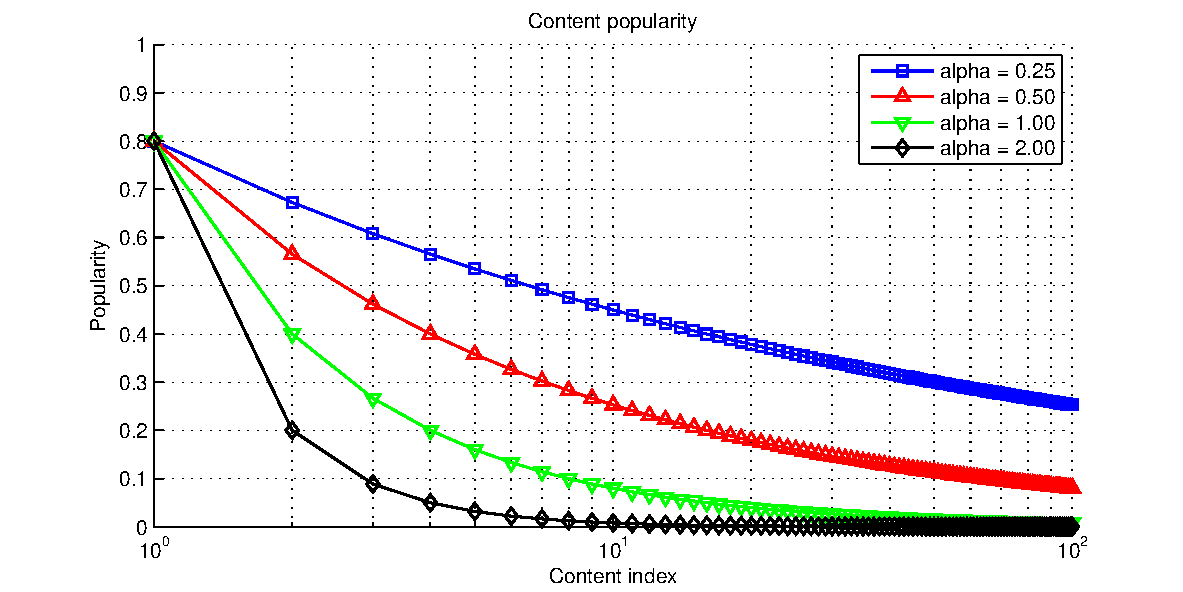
\includegraphics[width=0.40\textwidth]{figures/pop.pdf}
    \cprotect\caption{Content popularity distribution, for $c = 0.8$ and 
        $\alpha \in \{0.25, 0.5, 1, 2\}$.}
    \label{fig:zipf}

\end{figure}

At each experiment round (see Section~\ref{subsec:meth-conn-dots} for more details on 
rounds), each client $C$ generates a signal for content object $O_o$ with 
probability $q_{o}$. We consider a number of rounds 
$|N| = 10000$ for all experiment runs.\shortvertbreak

\subsubsection{Network Topologies}
\label{subsec:exp-setup-nettop}

We consider two types of topologies: (1) a cascade topology with $|L| = 5$ levels 
($|C| = 1$, $|R| = 1$ and $|S| = 1$), shown in Figure~\ref{fig:exp-setup-nettop-cascade}; (2) a binary 
tree topology, also with $|L| = 5$ levels ($|C| = 8$, $|R| = 7$ and $|S| = 1$), as 
shown in Figure~\ref{fig:exp-setup-nettop-tree}.\shortvertbreak

\begin{figure}[h!]
    \centering
    \subfigure[]{
        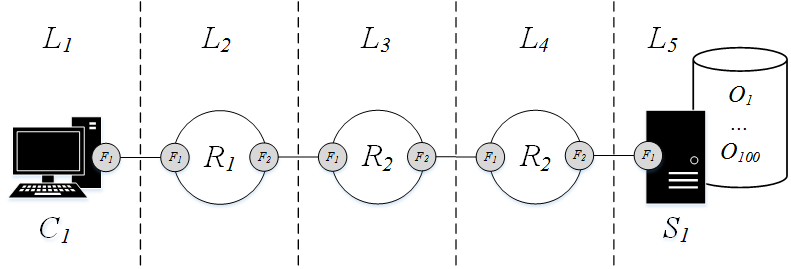
\includegraphics[width=0.30\textwidth] {figures/exp-setup-nettop-cascade.png}
        %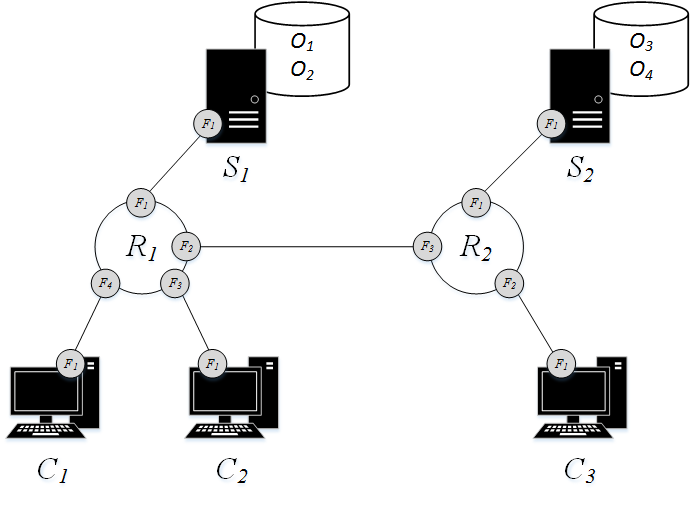
\includegraphics[width=0.30\textwidth] {figures/fib-topo.png}
        \label{fig:exp-setup-nettop-cascade}
    }

    \subfigure[]{
        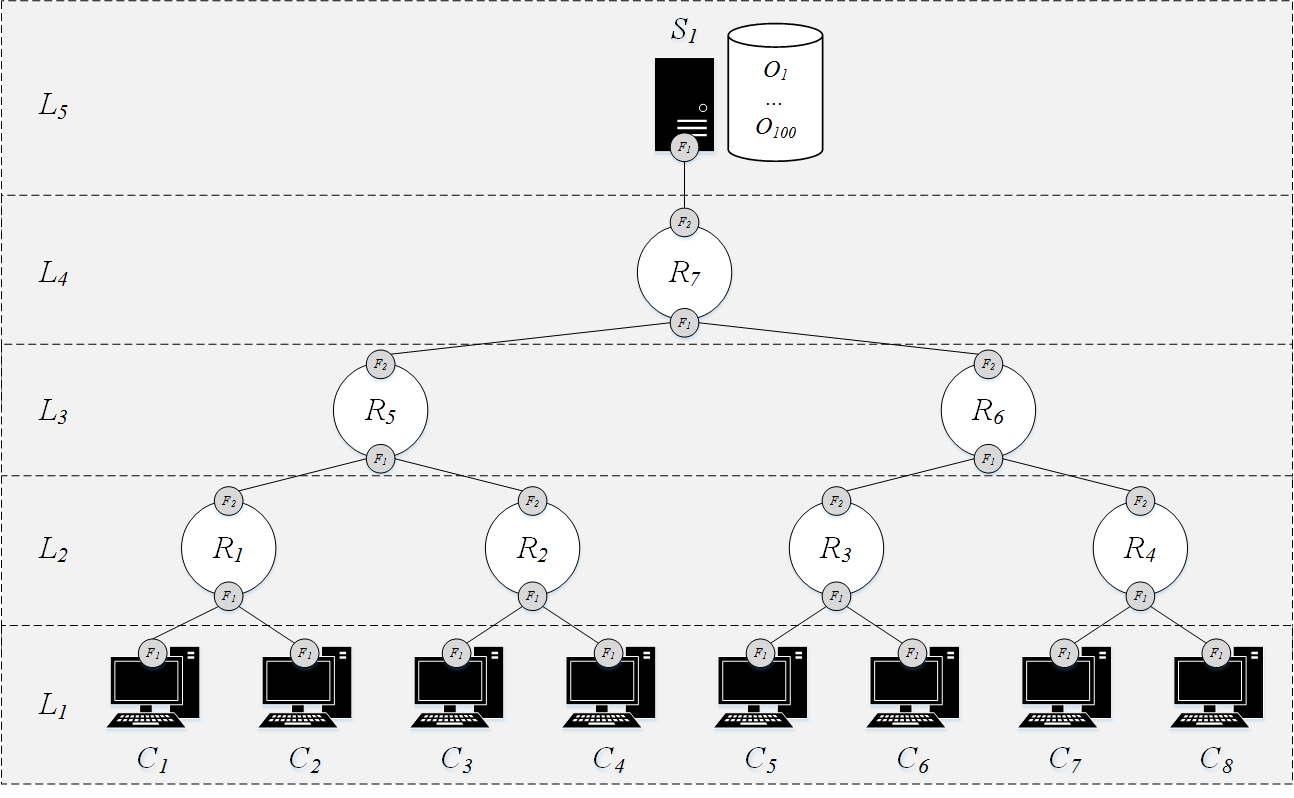
\includegraphics[width=0.40\textwidth] {figures/exp-setup-nettop-tree.png}
        %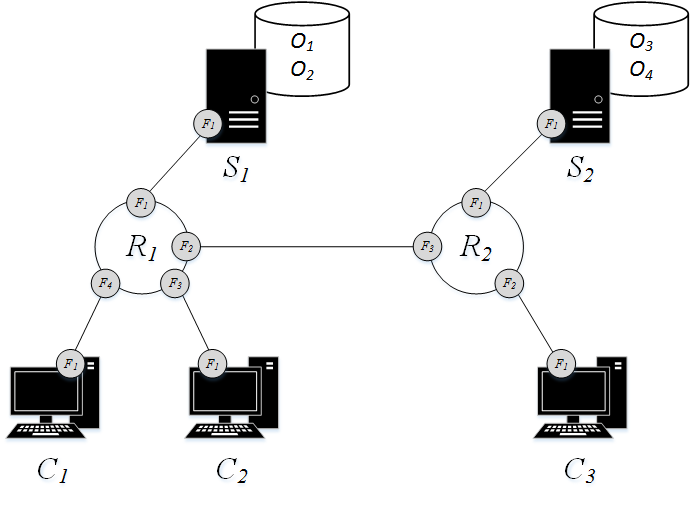
\includegraphics[width=0.30\textwidth] {figures/fib-topo.png}
        \label{fig:exp-setup-nettop-tree}
    }

    \cprotect\caption{Graphical depiction of the topologies considered for 
        our experiments: (a) cascade topology ($|L| = 5$, $|C| = 1$, $|R| = 3$ 
        and $|S| = 1$); (b) binary tree topology 
        ($|L| = 5$, $|C| = 8$, $|R| = 7$ and $|S| = 1$).}
    \label{fig:exp-setup-nettop}

\end{figure}

The definition of `topology level' is straightforward and depicted 
in Figure~\ref{fig:exp-setup-nettop}. Furthermore, we set the FIBs of every 
NDN router to forward Interests over the upstream interfaces, i.e. $F_{r,2}$, 
resulting in the form:

\begin{equation}
\textbf{FIB} = \begin{bmatrix} 
                0 & 1 & 0 & ... & 0                 \\ 
                0 & 1 & 0 & ... & 0                 \\ 
                ... & ... & ... & ... & ...         \\ 
                0 & 1 & 0 & ... & 0                 \\ \end{bmatrix}
    \label{eq:fib-exp}
\end{equation}\shortvertbreak

\subsubsection{Cache Characteristics}
\label{subsec:exp-setup-cache}

We evaluate the performance of our model under three different types of cache 
algorithms, already described in Section~\ref{subsec:meth-caching-algs}: (1) 
Least Recently Used (LRU); (2) More Recently Used (MRU); and (3) Random caching. We 
consider different cache sizes, specifically $|P| = \{10, 25, 50, 75\}$.\shortvertbreak

\subsubsection{Metrics}
\label{subsec:exp-setup-metrics}

For all our experiments we collect and evaluate the following metrics:

\begin{enumerate}

    \item Total number of Interests and Data packets received\slash sent per network node\slash level;
    \item Cache hit\slash miss rate per content object and network level;
    \item Ratio of received Interests to original requests, per content object 
        and network level (including server(s) $S$);
    \item Relative time spent at cache per content object.\shortvertbreak

\end{enumerate}

Regarding metric 2, we first provide our definition of `cache hit': a cache hit 
happens when an Interest signal for some content object $O_o$, arriving at some 
router $R_r$, finds a cached copy of $O_o$ at the CS of $R_r$. Therefore, to 
compute metric 2, we consider the Interest signals 
arriving at all NDN routers of some level $L$, discriminated by content 
object $O_o$, for all simulation rounds $N$. We then find the ratio between Interest 
`hits' for $O_o$, $i'_{O_o}$, and the total value of arriving Interests for $O_o$ at that 
level, $i_{O_o}$:

\begin{equation}
    \frac{\sum_{n=1}^{|N|} i'_{O_o}}{\sum_{n=1}^{|N|} i_{O_o}} \quad \forall \ R_r \ \text{in level $L$}
    \label{eq:exp-setup-metrics-2}
\end{equation}\shortvertbreak

For metric 4, we simply find the average number of rounds 
some content object $O_o$ spends at the caches of NDN routers of some level $L$, and find 
the ratio vs. the total number of simulation rounds.

\subsection{Experimental Results}
\label{subsec:exp-results}

Here we present a selection of experimental results, following the metrics 
introduced in Section~\ref{subsec:exp-setup}\footnote{A complete collection of 
results can be found in~\url{github.com/adamiaonr/mtsp-project/tree/master/report/figures/experiments}.}. 
The captions on the figures enclose the respective experimental parameters.\shortvertbreak

%\subsubsection{Network Topologies}
%\label{subsec:exp-results-topologies}

\begin{figure}[h!]
    \centering

    \subfigure[]{
        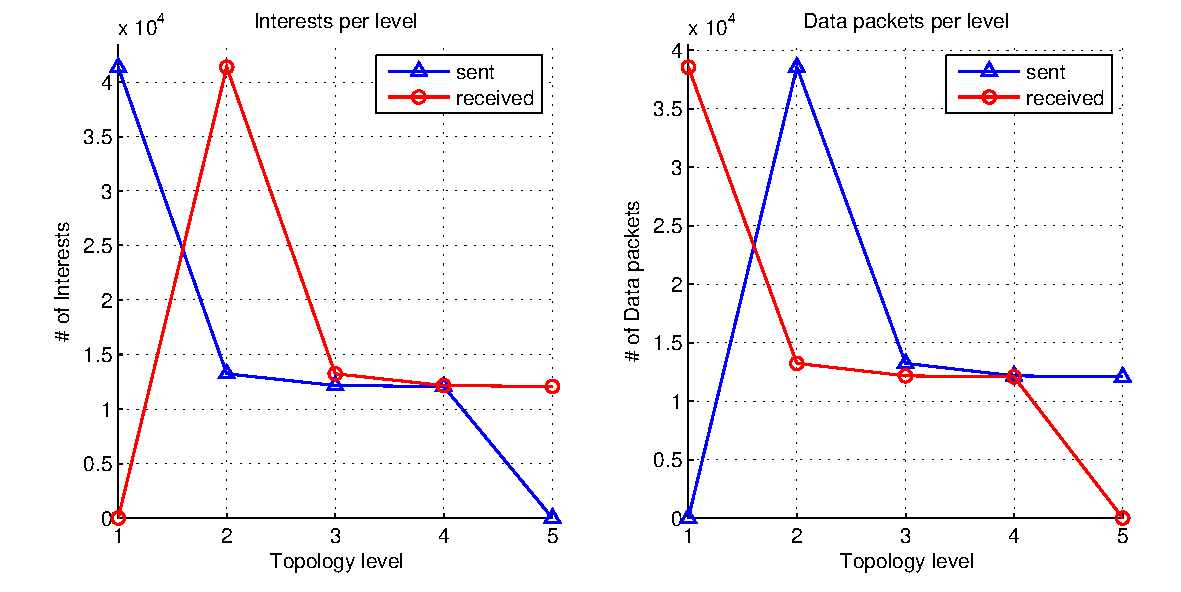
\includegraphics[width=0.40\textwidth] {figures/experiments/cascade/LRU/25/6-2.pdf}
        %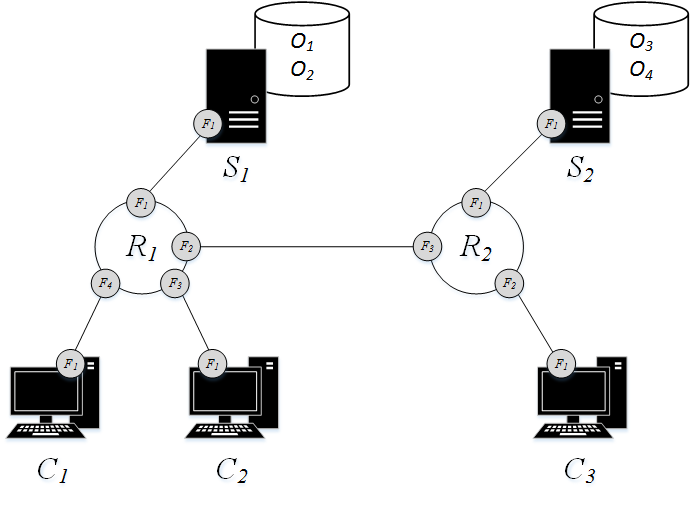
\includegraphics[width=0.30\textwidth] {figures/fib-topo.pdf}
        \label{fig:exp-results-topologies-cascade-lru}
    }

    \subfigure[]{
        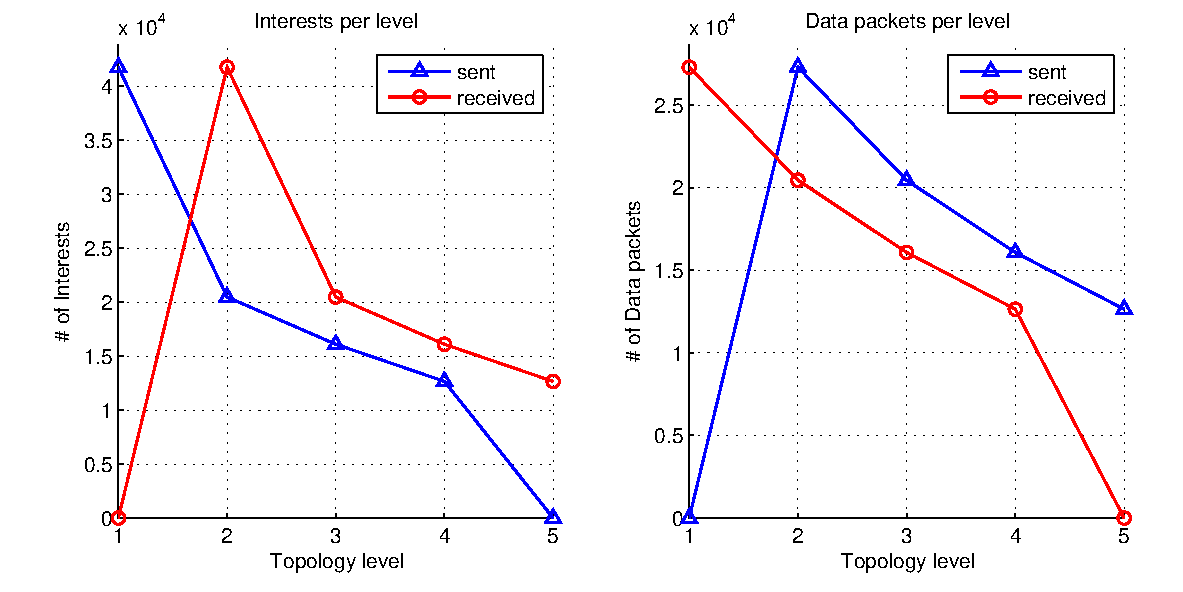
\includegraphics[width=0.40\textwidth] {figures/experiments/cascade/MRU/25/6-2.pdf}
        %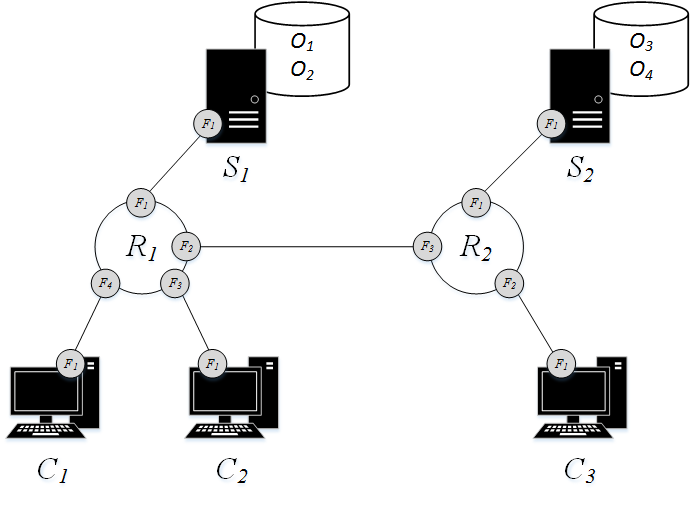
\includegraphics[width=0.30\textwidth] {figures/fib-topo.pdf}
        \label{fig:exp-results-topologies-cascade-mru}
    }

    \cprotect\caption{Number of Interests\slash Data packets sent\slash received 
        per topology level, for different cache algorithms: LRU (a), MRU (b). 
        Cascade topology, $|P| = 25$, $\alpha = 1$, LRU caching.}
    \label{fig:exp-results-topologies-cascade}

\end{figure}

\begin{figure}[h!]
    \centering

    \subfigure[]{
        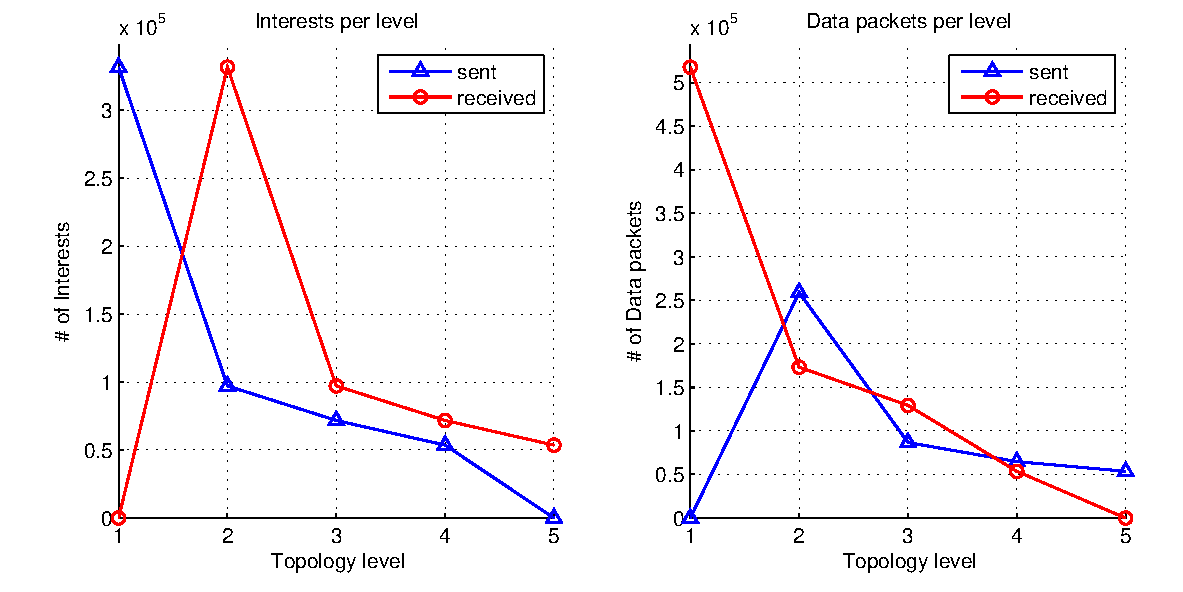
\includegraphics[width=0.40\textwidth] {figures/experiments/tree/LRU/25/6-2.pdf}
        %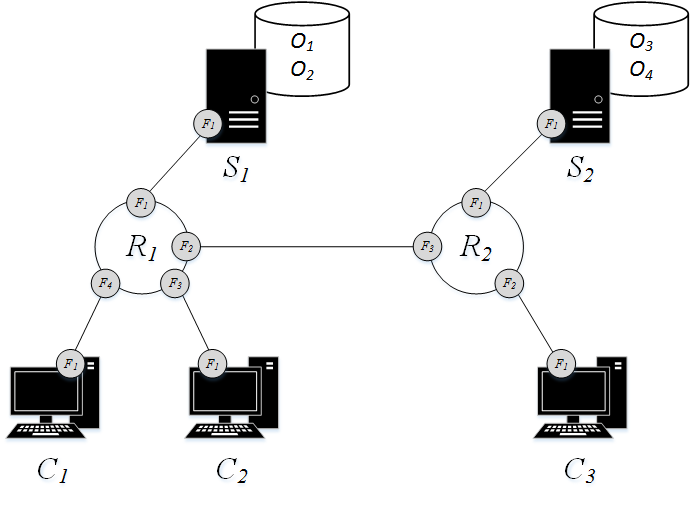
\includegraphics[width=0.30\textwidth] {figures/fib-topo.pdf}
        \label{fig:exp-results-topologies-tree-lru}
    }

    \subfigure[]{
        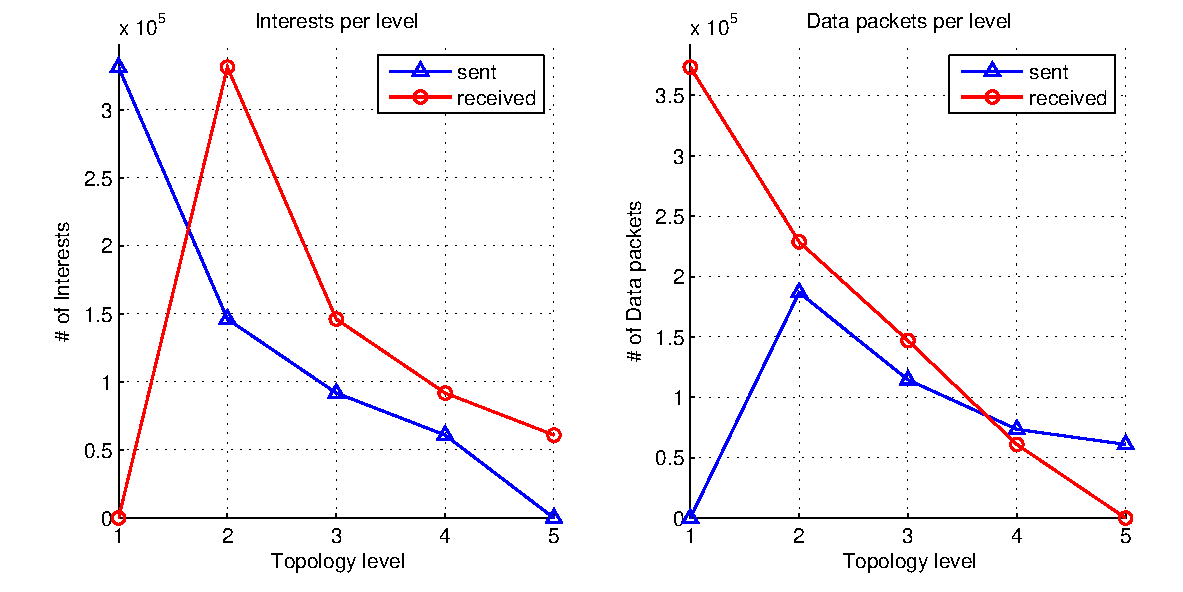
\includegraphics[width=0.40\textwidth] {figures/experiments/tree/MRU/25/6-2.pdf}
        %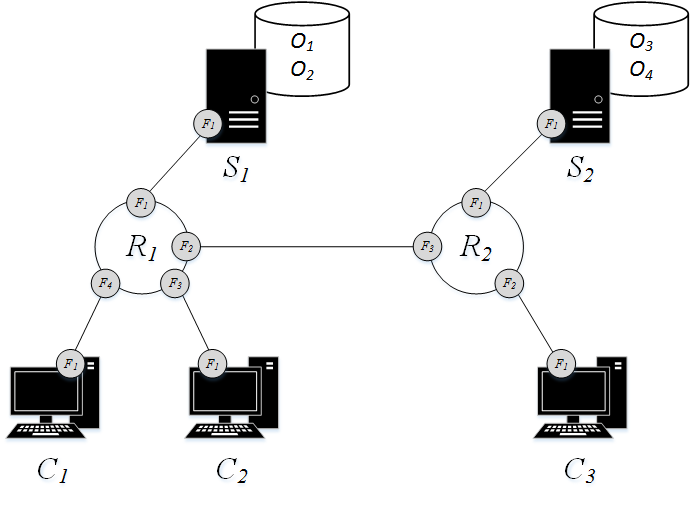
\includegraphics[width=0.30\textwidth] {figures/fib-topo.pdf}
        \label{fig:exp-results-topologies-tree-mru}
    }

    \cprotect\caption{Number of Interests\slash Data packets sent\slash received 
        per topology level, for different cache algorithms: LRU (a), MRU (b). 
        Binary tree topology, $|P| = 25$, $\alpha = 1$, MRU caching.}
    \label{fig:exp-results-topologies-tree}

\end{figure}

%\subsubsection{Cache Algorithms}
%\label{subsec:exp-results-cache-alg}

\begin{figure}[h!]
    \centering
    \subfigure[]{
        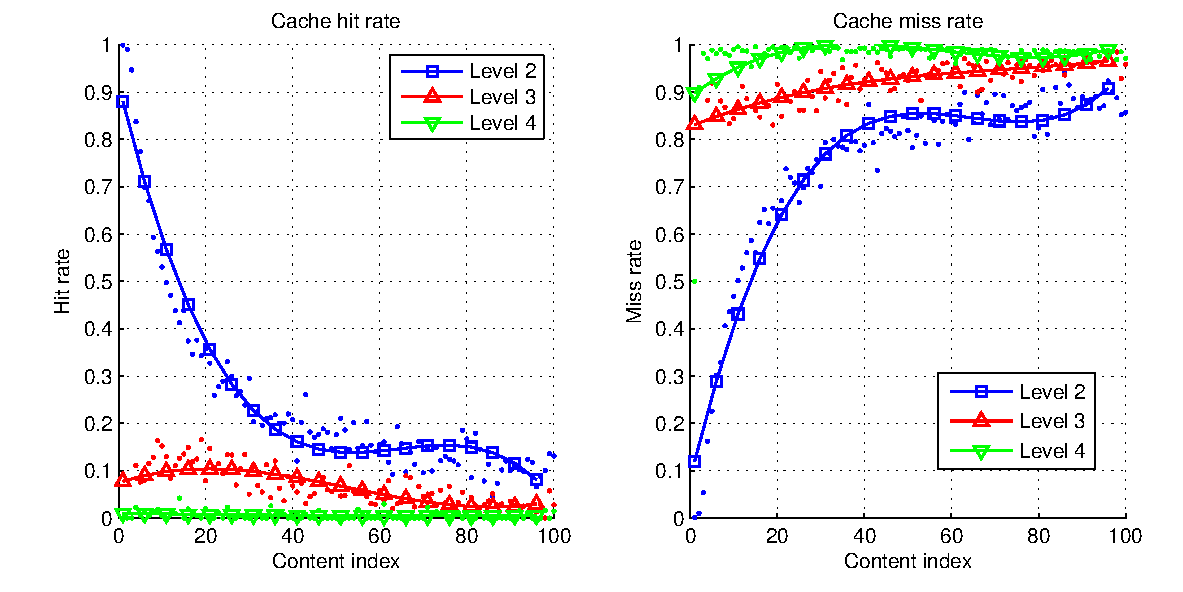
\includegraphics[width=0.40\textwidth] {figures/experiments/cascade/LRU/25/6-3.pdf}
        %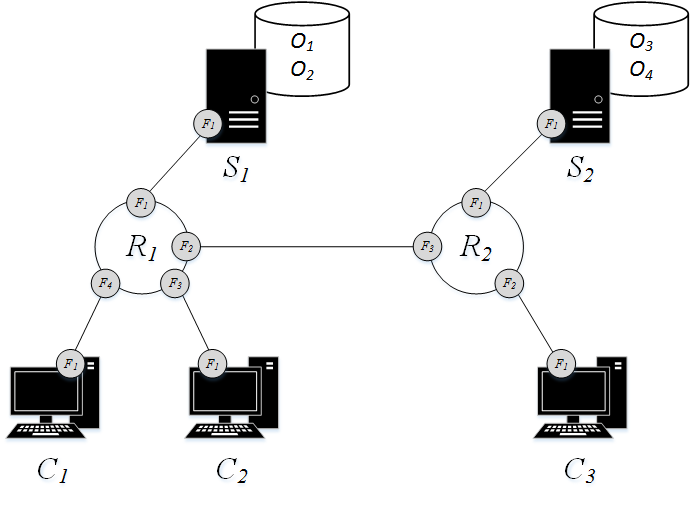
\includegraphics[width=0.30\textwidth] {figures/fib-topo.pdf}
        \label{fig:exp-results-cache-alg-cascade-lru}
    }

    \subfigure[]{
        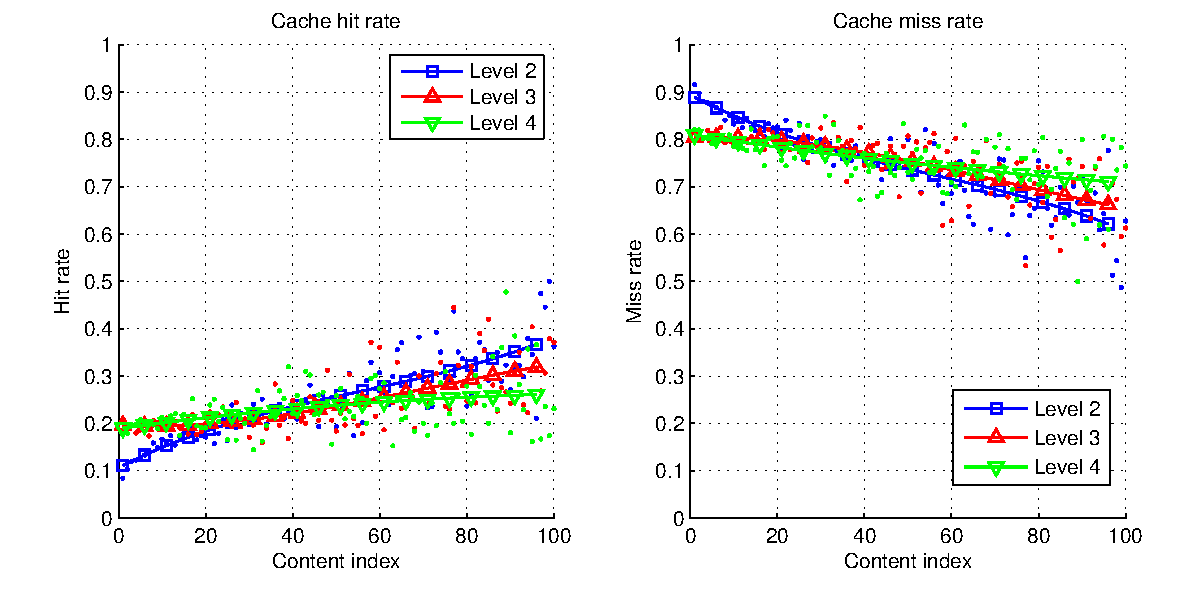
\includegraphics[width=0.40\textwidth] {figures/experiments/cascade/MRU/25/6-3.pdf}
        %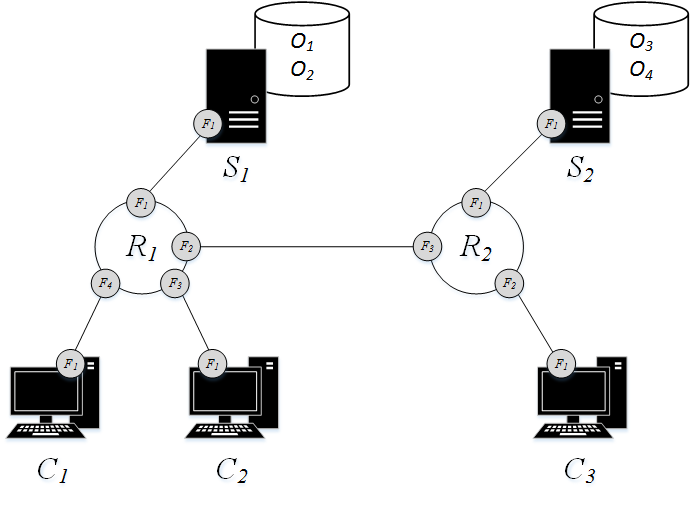
\includegraphics[width=0.30\textwidth] {figures/fib-topo.pdf}
        \label{fig:exp-results-cache-alg-cascade-mru}
    }

    \subfigure[]{
        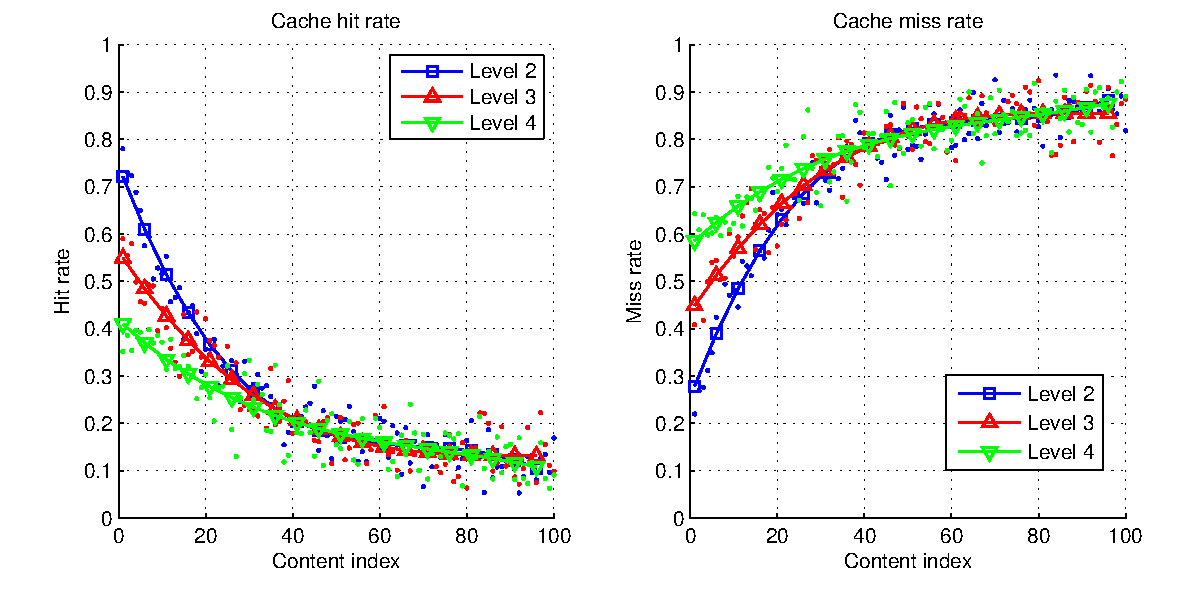
\includegraphics[width=0.40\textwidth] {figures/experiments/cascade/RANDOM/25/6-3.pdf}
        %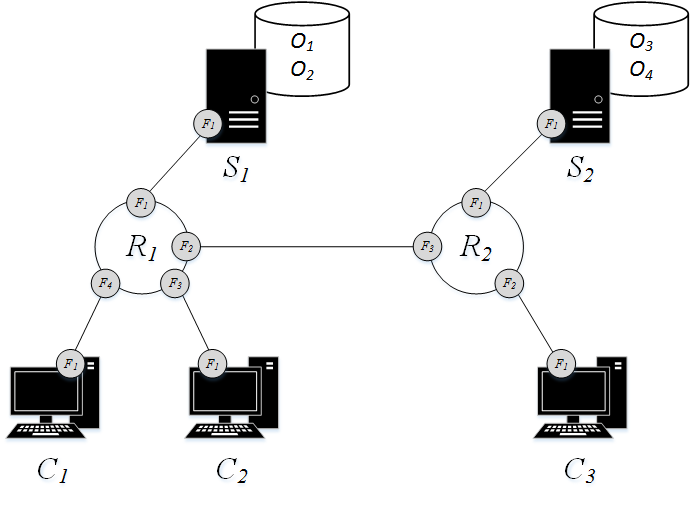
\includegraphics[width=0.30\textwidth] {figures/fib-topo.pdf}
        \label{fig:exp-results-cache-alg-cascade-random}
    }

    \cprotect\caption{Cache hit\slash miss rates for different cache algorithms: LRU (a), MRU (b) 
        and Random caching (c). Cascade topology, $|L| = 5$, $|C| = 1$, 
        $|R| = 3$ and $|S| = 1$, $|P| = 25$, $\alpha = 1$.}
    \label{fig:exp-results-cache-alg-cascade}

\end{figure}

\begin{figure}[h!]
    \centering
    \subfigure[]{
        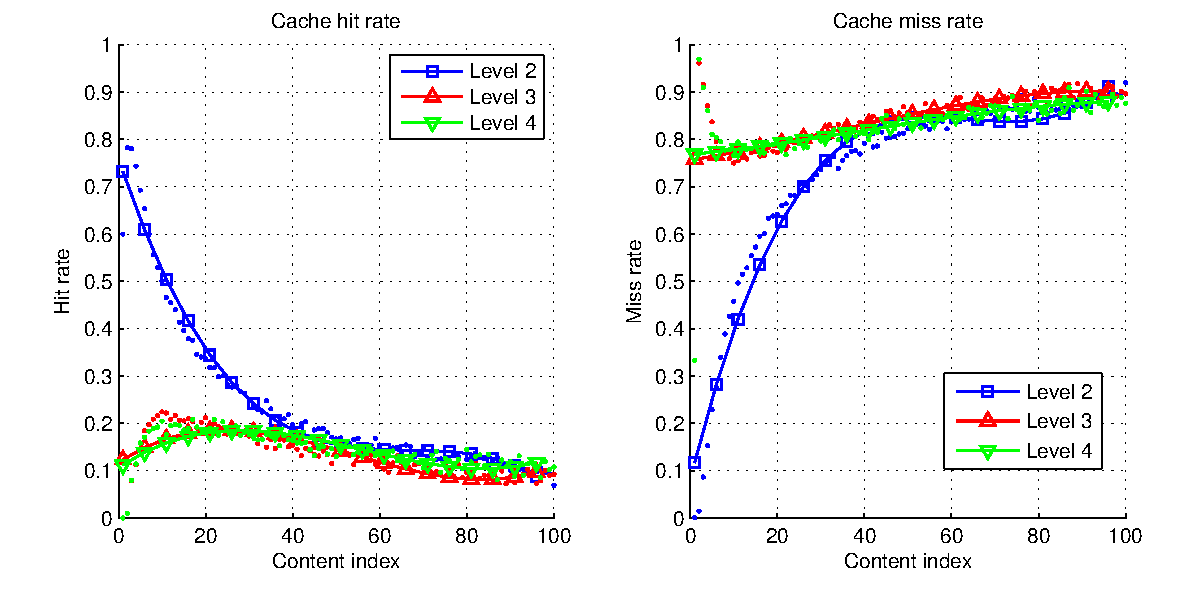
\includegraphics[width=0.40\textwidth] {figures/experiments/tree/LRU/25/6-3.pdf}
        %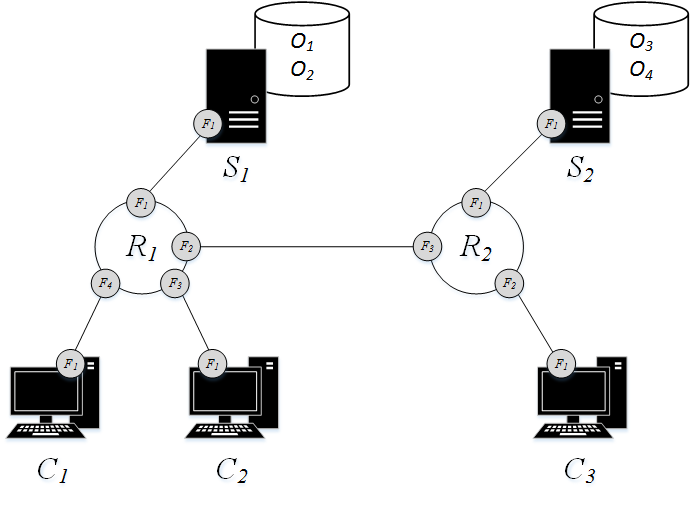
\includegraphics[width=0.30\textwidth] {figures/fib-topo.pdf}
        \label{fig:exp-results-cache-alg-tree-lru}
    }

    \subfigure[]{
        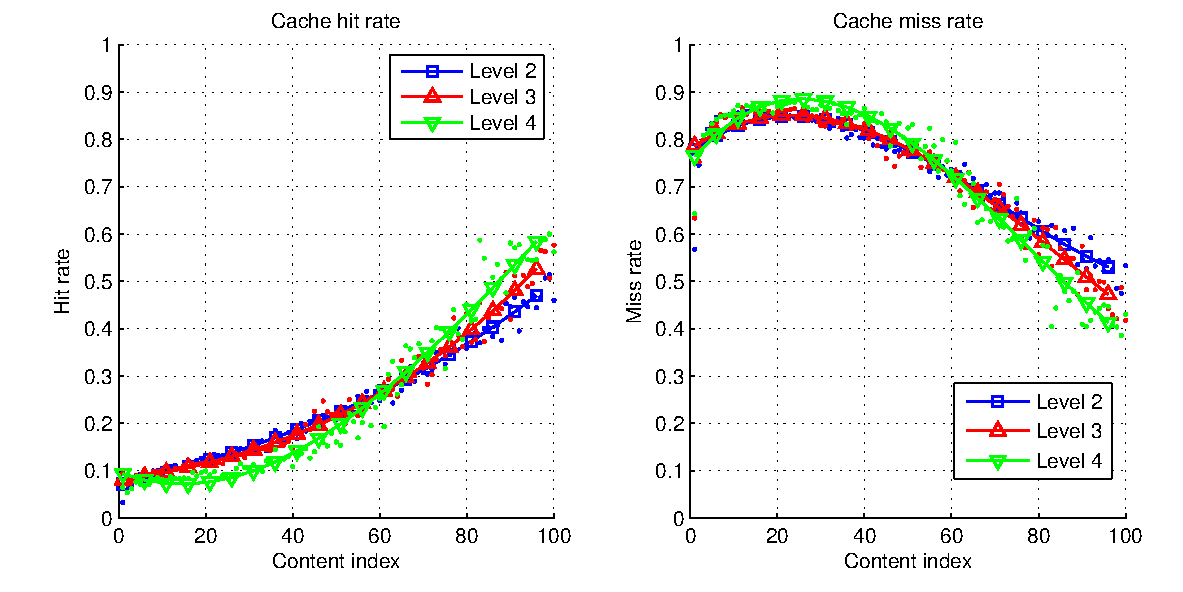
\includegraphics[width=0.40\textwidth] {figures/experiments/tree/MRU/25/6-3.pdf}
        %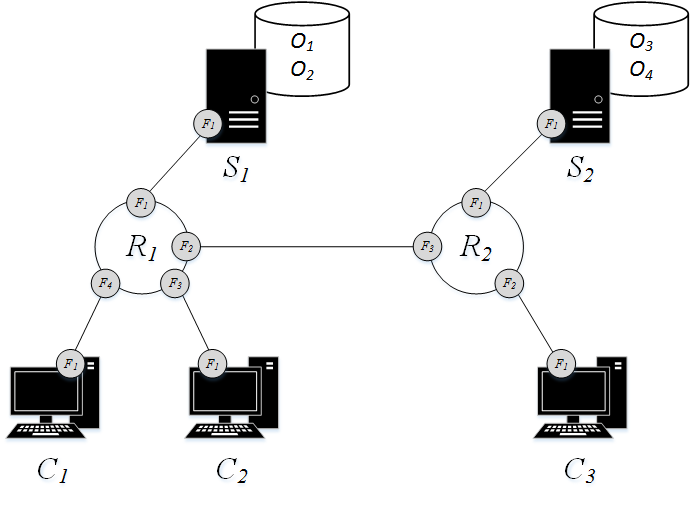
\includegraphics[width=0.30\textwidth] {figures/fib-topo.pdf}
        \label{fig:exp-results-cache-alg-tree-mru}
    }

    \subfigure[]{
        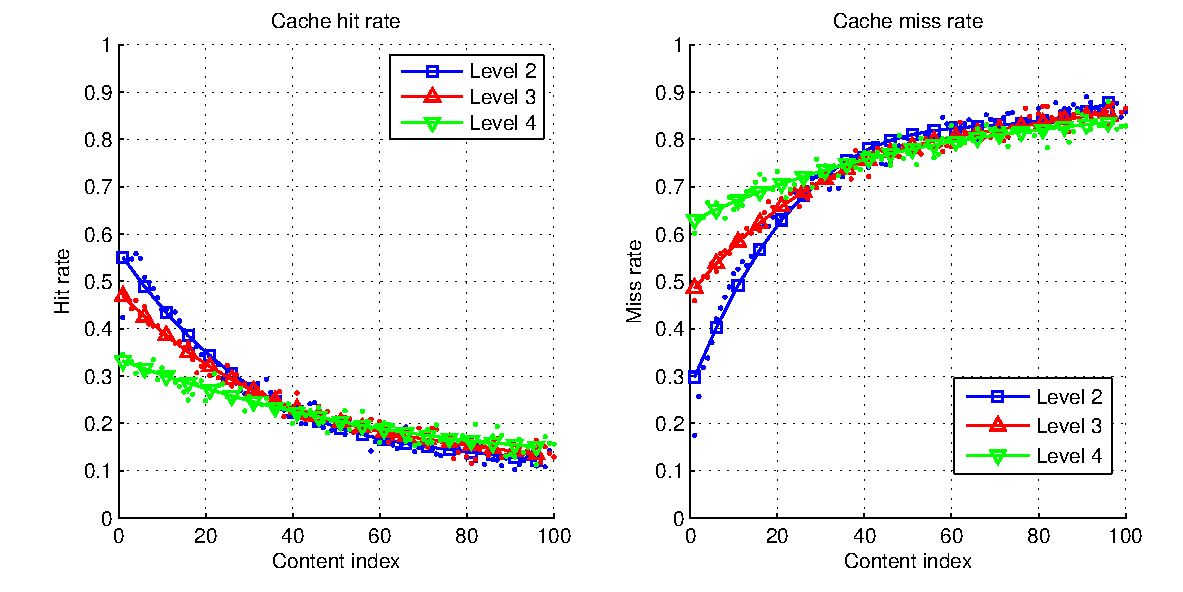
\includegraphics[width=0.40\textwidth] {figures/experiments/tree/RANDOM/25/6-3.pdf}
        %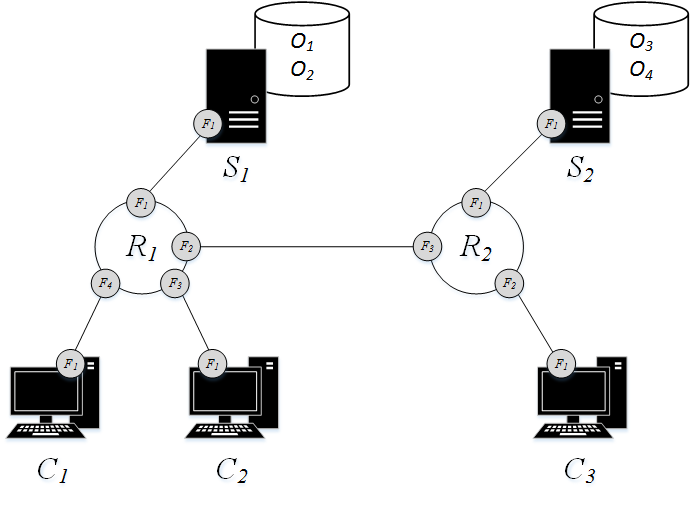
\includegraphics[width=0.30\textwidth] {figures/fib-topo.pdf}
        \label{fig:exp-results-cache-alg-tree-random}
    }

    \cprotect\caption{Cache hit\slash miss rates for different cache algorithms: LRU (a), MRU (b) 
        and Random caching (c). Binary tree topology, $|L| = 5$, $|C| = 8$, 
        $|R| = 7$ and $|S| = 1$, $|P| = 25$, $\alpha = 1$.}
    \label{fig:exp-results-cache-alg-tree}

\end{figure}

\begin{figure}[h!]
    \centering
    \subfigure[]{
        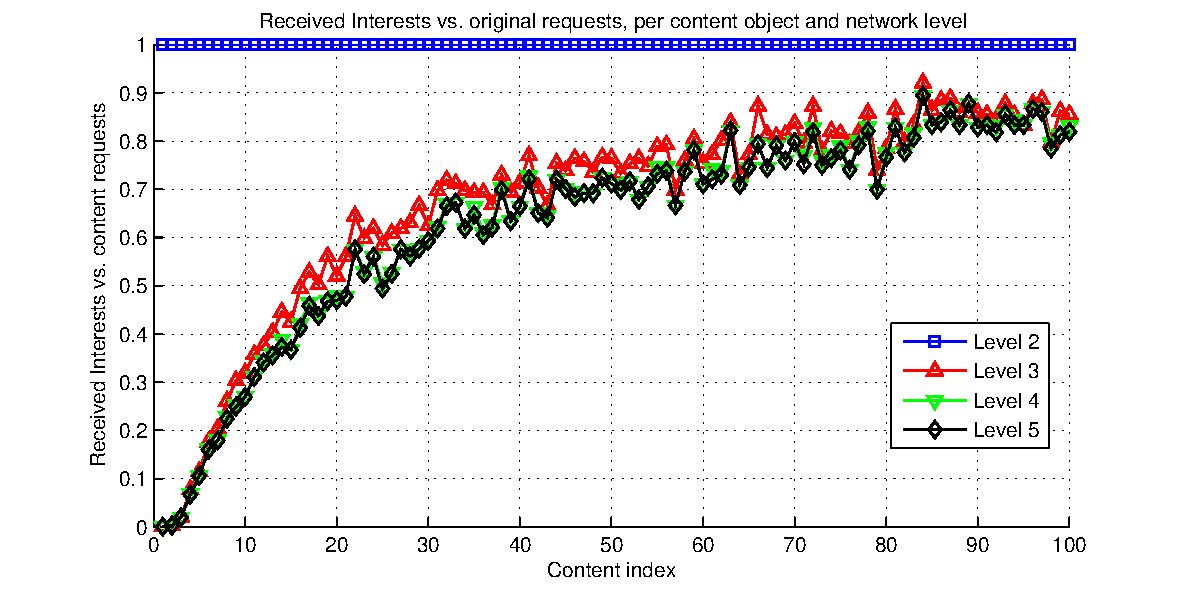
\includegraphics[width=0.40\textwidth] {figures/experiments/cascade/LRU/25/6-5.pdf}
        %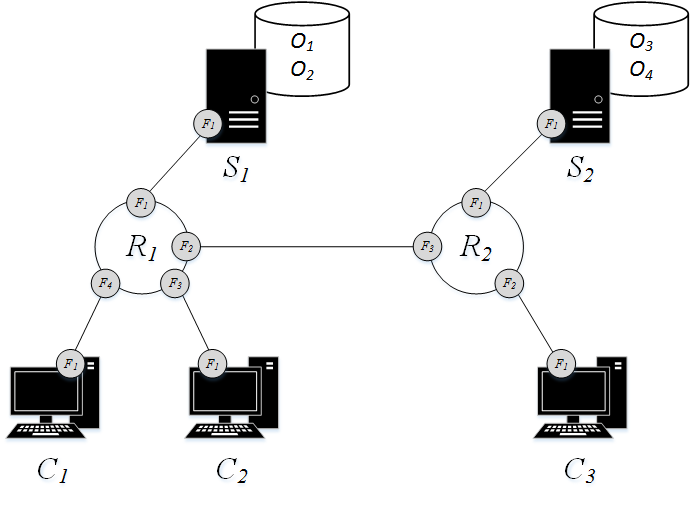
\includegraphics[width=0.30\textwidth] {figures/fib-topo.pdf}
        \label{fig:exp-results-latency-cascade-lru}
    }

    \subfigure[]{
        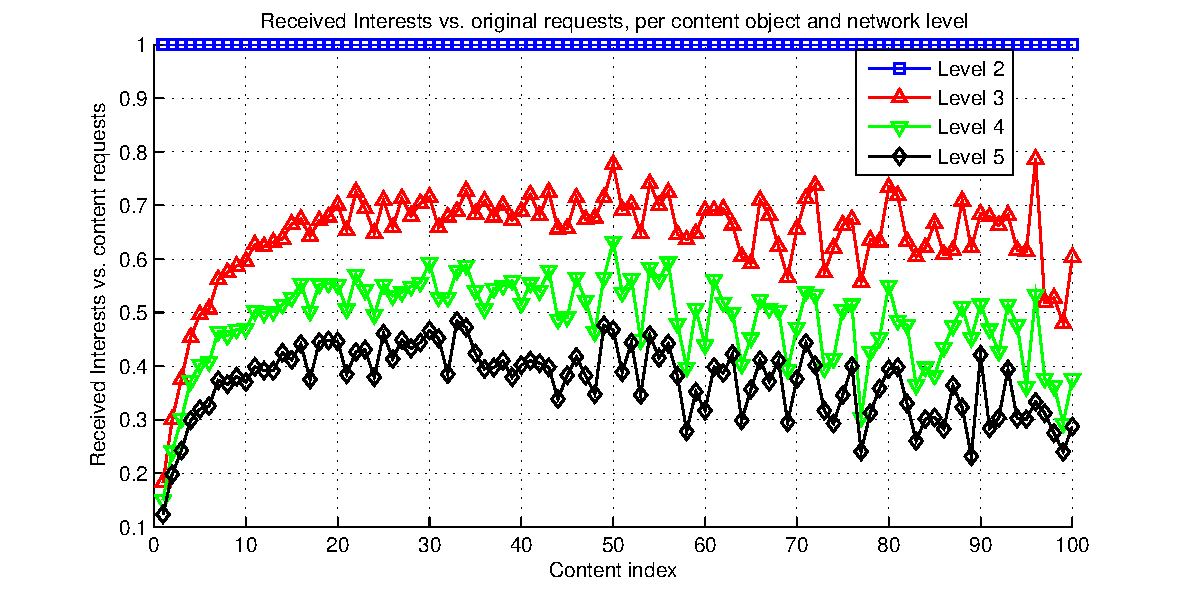
\includegraphics[width=0.40\textwidth] {figures/experiments/cascade/MRU/25/6-5.pdf}
        %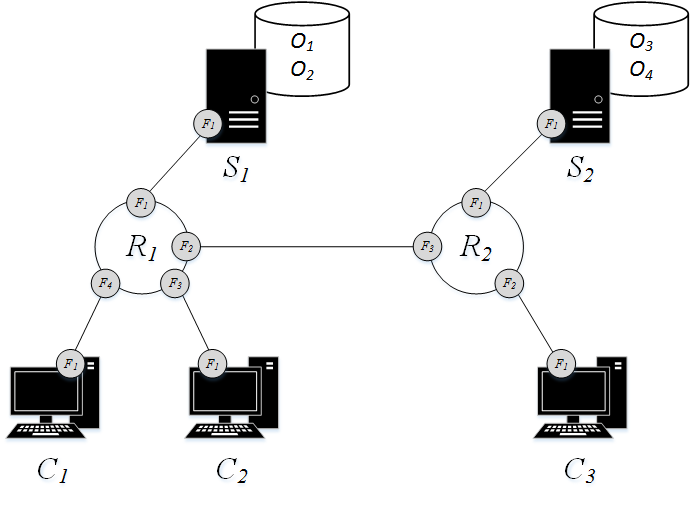
\includegraphics[width=0.30\textwidth] {figures/fib-topo.pdf}
        \label{fig:exp-results-latency-cascade-mru}
    }

    \subfigure[]{
        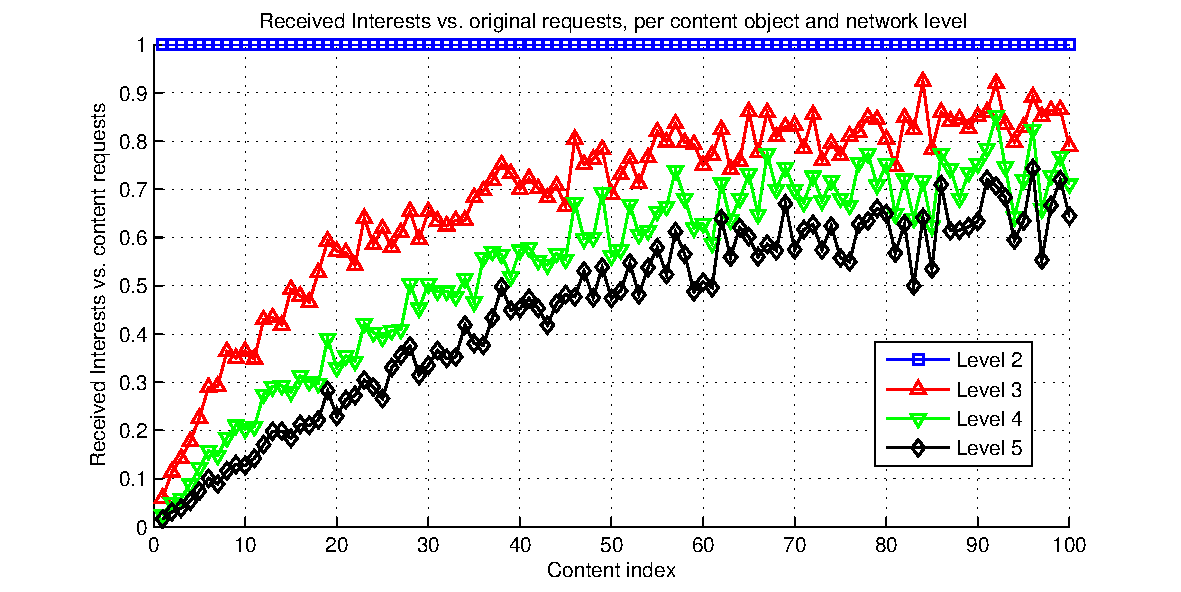
\includegraphics[width=0.40\textwidth] {figures/experiments/cascade/RANDOM/25/6-5.pdf}
        %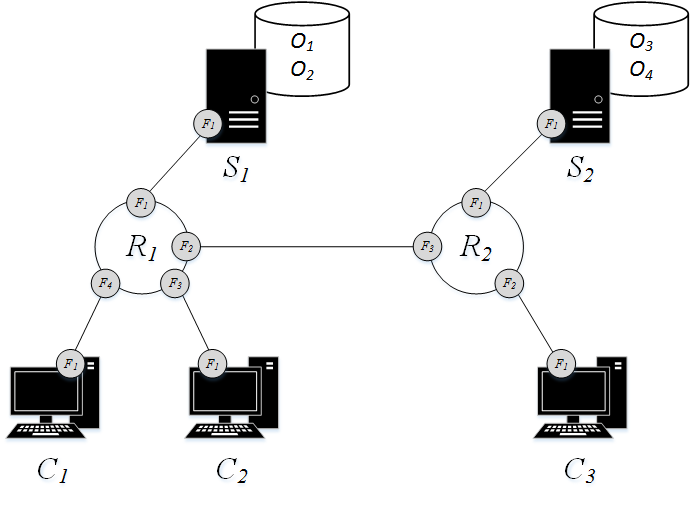
\includegraphics[width=0.30\textwidth] {figures/fib-topo.pdf}
        \label{fig:exp-results-latency-cascade-random}
    }

    \cprotect\caption{Received Interests to original requests ratio, per content 
        object and network level. Different cache algorithms --- LRU (a), MRU (b) and 
        random caching (c) --- cascade topology, $|L| = 5$, $|C| = 1$, 
        $|R| = 3$ and $|S| = 1$, $|P| = 25$, $\alpha = 1$.}
    \label{fig:exp-results-latency-cascade}

\end{figure}

\begin{figure}[h!]
    \centering
    \subfigure[]{
        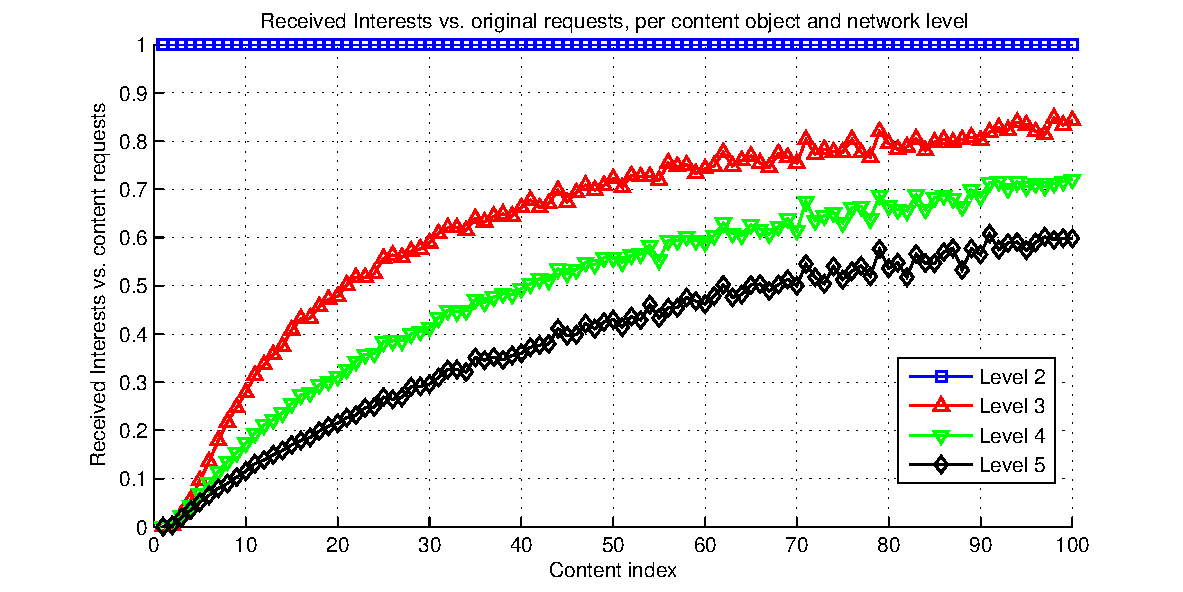
\includegraphics[width=0.40\textwidth] {figures/experiments/tree/LRU/25/6-5.pdf}
        %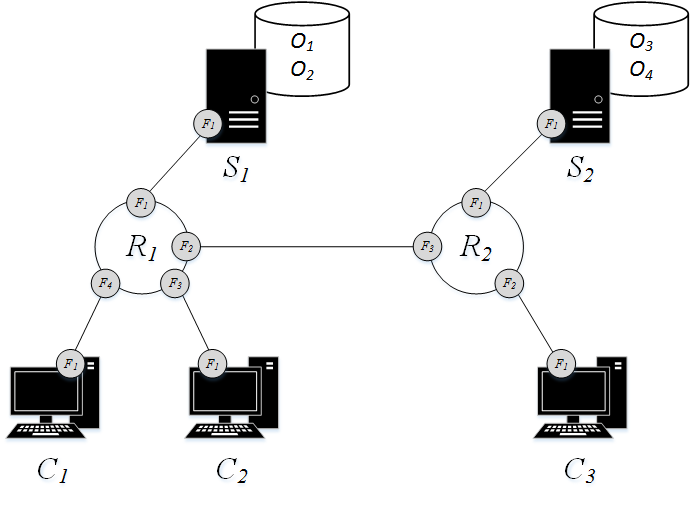
\includegraphics[width=0.30\textwidth] {figures/fib-topo.pdf}
        \label{fig:exp-results-latency-tree-lru}
    }

    \subfigure[]{
        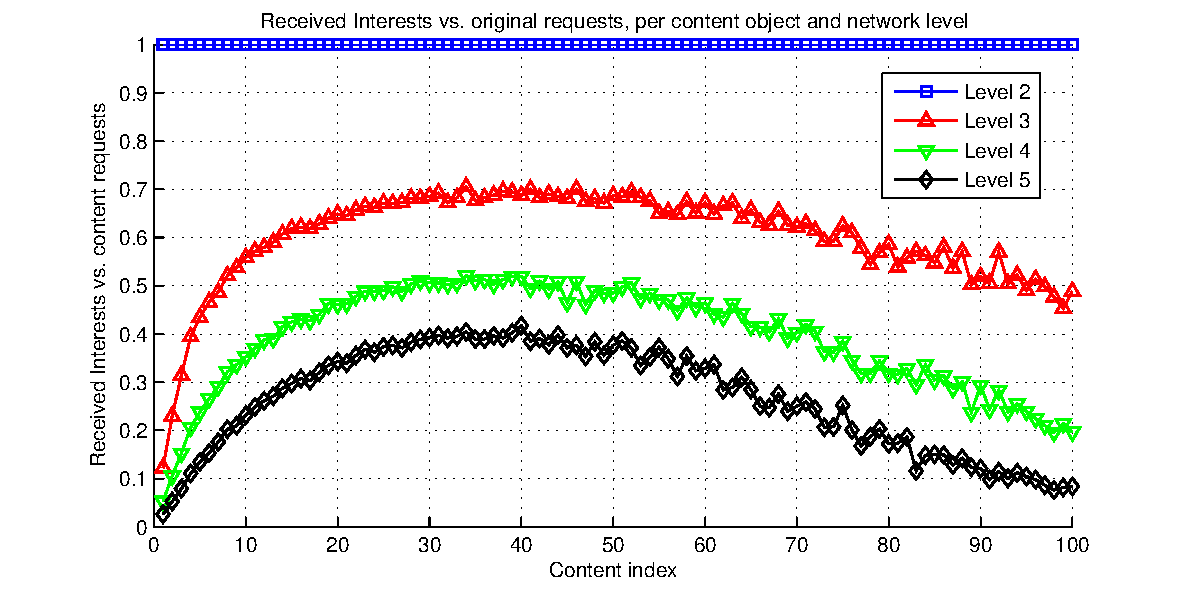
\includegraphics[width=0.40\textwidth] {figures/experiments/tree/MRU/25/6-5.pdf}
        %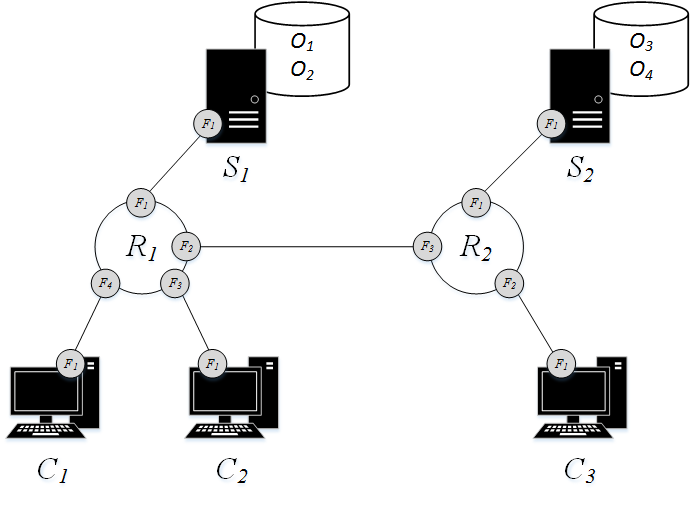
\includegraphics[width=0.30\textwidth] {figures/fib-topo.pdf}
        \label{fig:exp-results-latency-tree-mru}
    }

    \subfigure[]{
        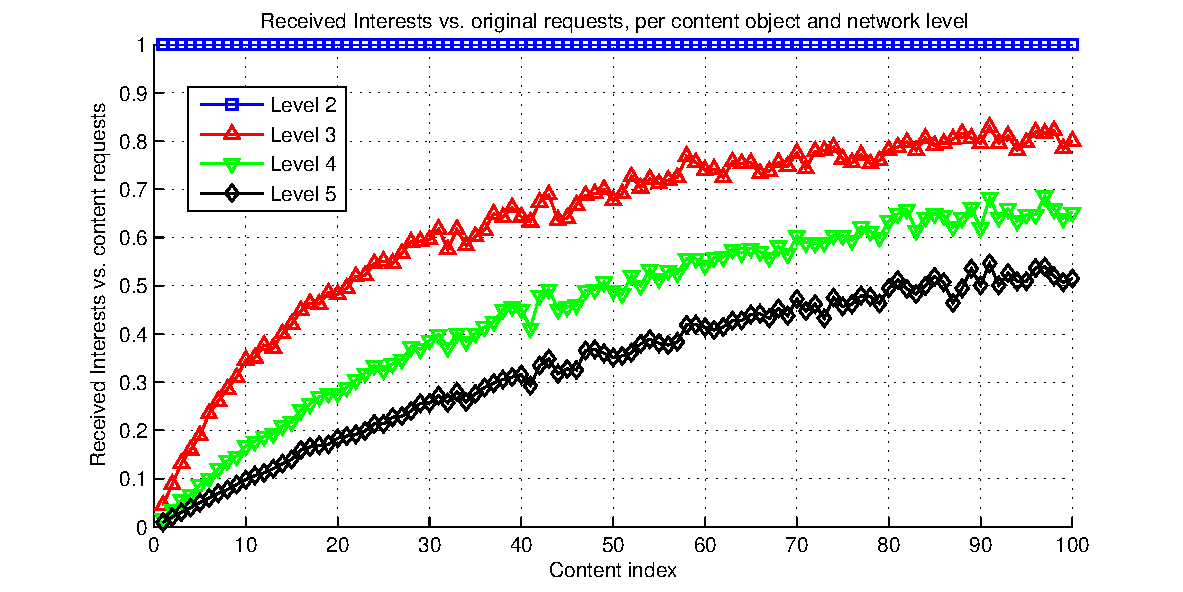
\includegraphics[width=0.40\textwidth] {figures/experiments/tree/RANDOM/25/6-5.pdf}
        %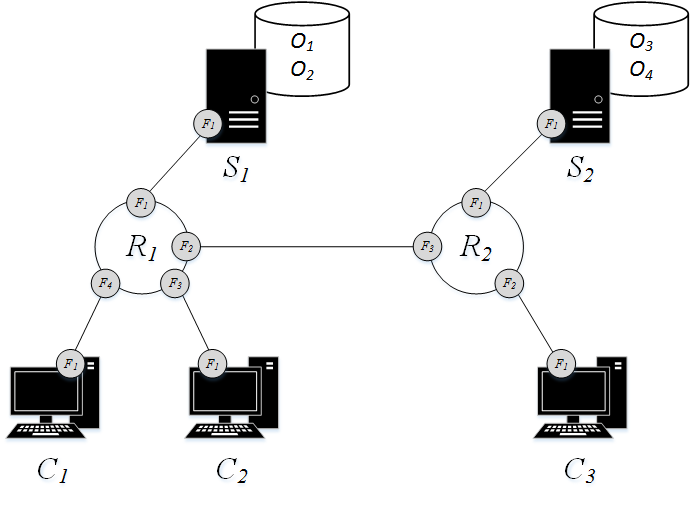
\includegraphics[width=0.30\textwidth] {figures/fib-topo.pdf}
        \label{fig:exp-results-latency-tree-random}
    }

    \cprotect\caption{Received Interests to original requests ratio, per content 
        object and network level. Different cache algorithms --- LRU (a), MRU (b) and 
        random caching (c) --- binary tree topology, $|L| = 5$, $|C| = 8$, 
        $|R| = 7$ and $|S| = 1$, $|P| = 25$, $\alpha = 1$.}
    \label{fig:exp-results-latency-tree}

\end{figure}

\begin{figure}[h!]
    \centering
    \subfigure[]{
        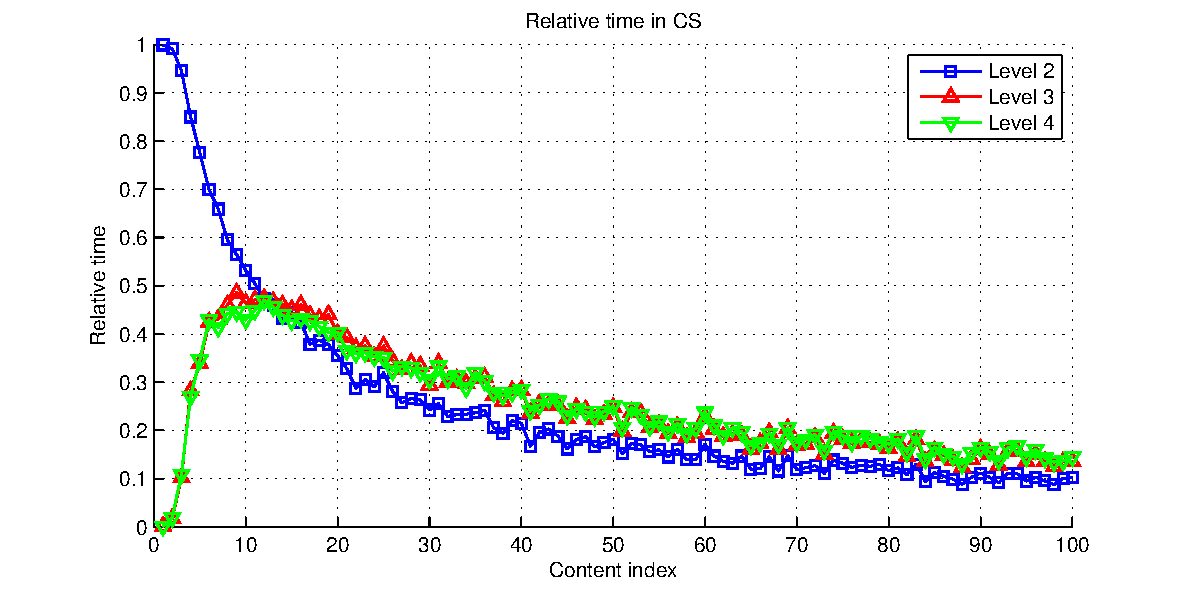
\includegraphics[width=0.40\textwidth] {figures/experiments/cascade/LRU/25/6-4.pdf}
        %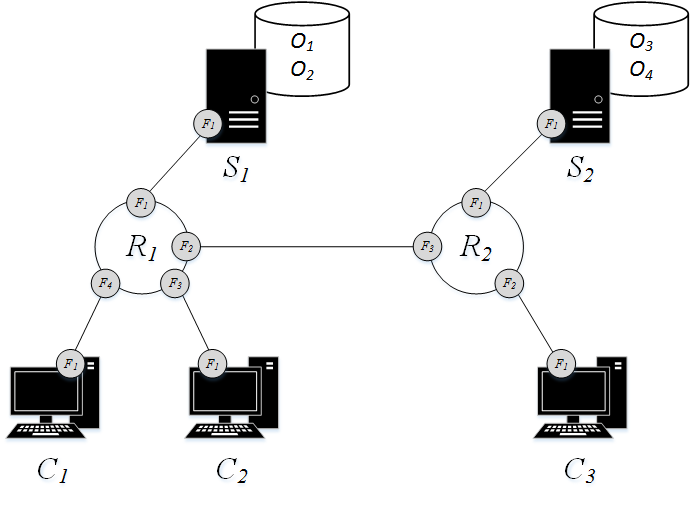
\includegraphics[width=0.30\textwidth] {figures/fib-topo.pdf}
        \label{fig:exp-results-time-cascade-lru}
    }

    \subfigure[]{
        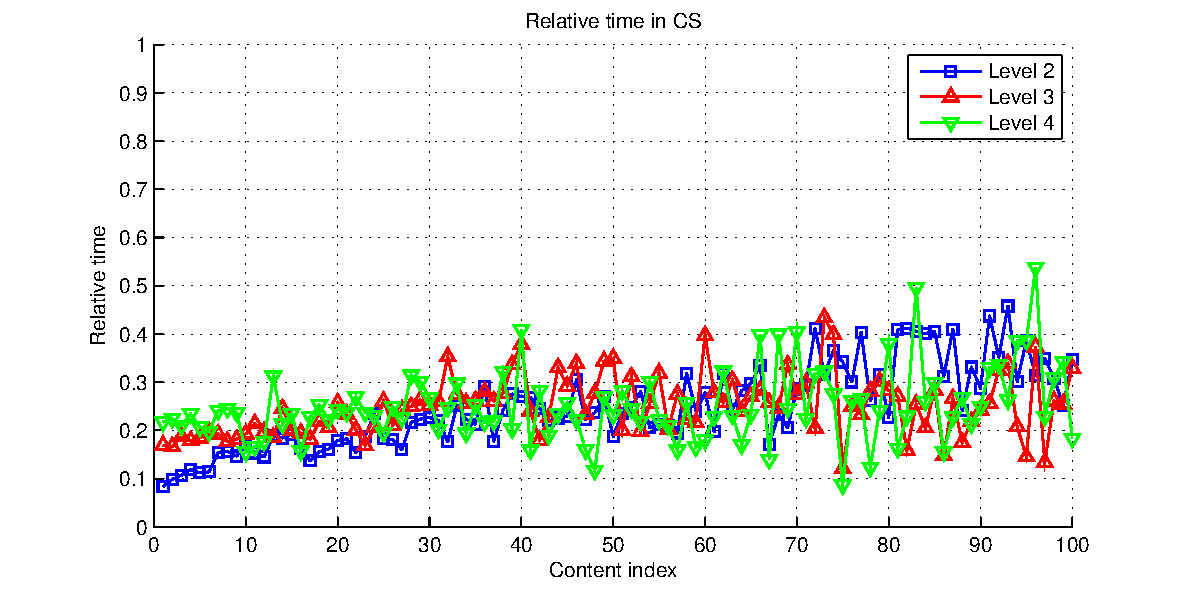
\includegraphics[width=0.40\textwidth] {figures/experiments/cascade/MRU/25/6-4.pdf}
        %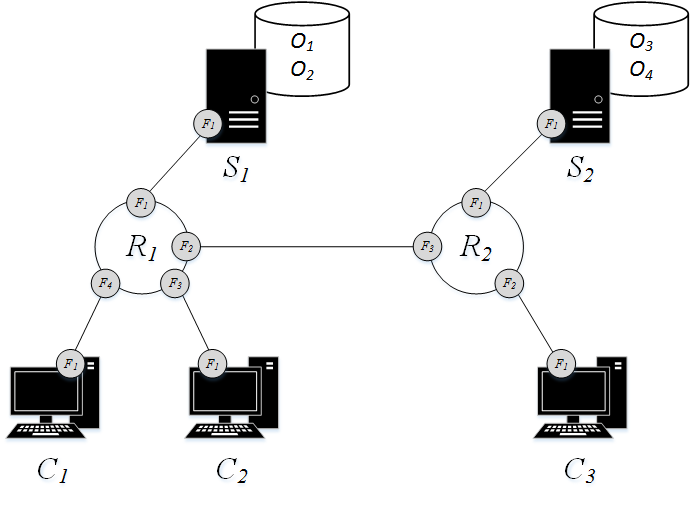
\includegraphics[width=0.30\textwidth] {figures/fib-topo.pdf}
        \label{fig:exp-results-time-cascade-mru}
    }

    \subfigure[]{
        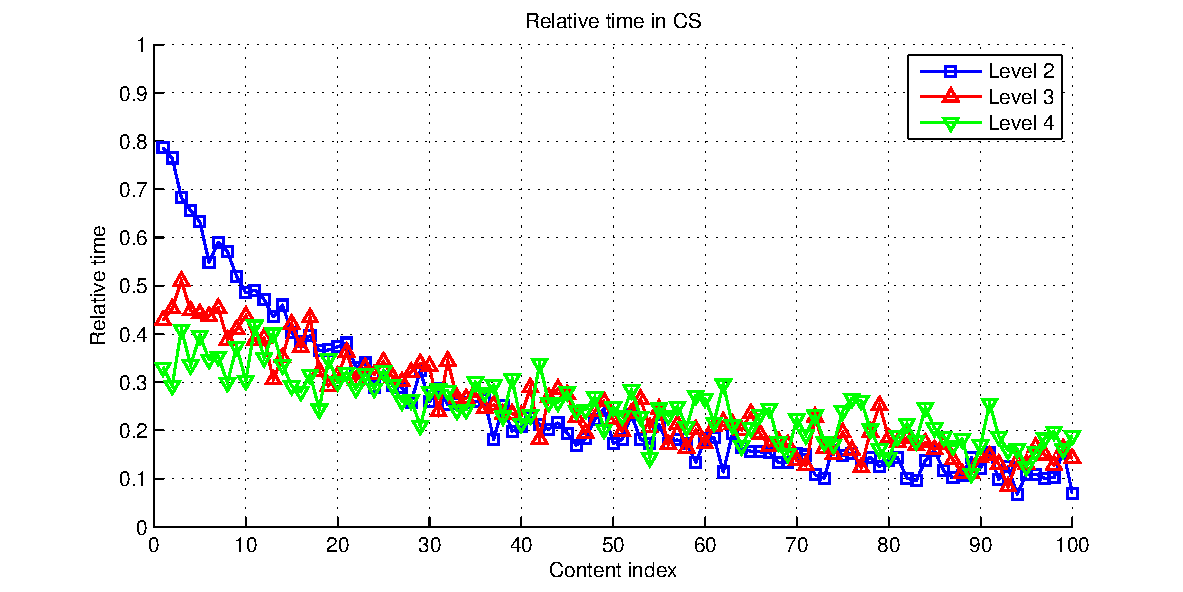
\includegraphics[width=0.40\textwidth] {figures/experiments/cascade/RANDOM/25/6-4.pdf}
        %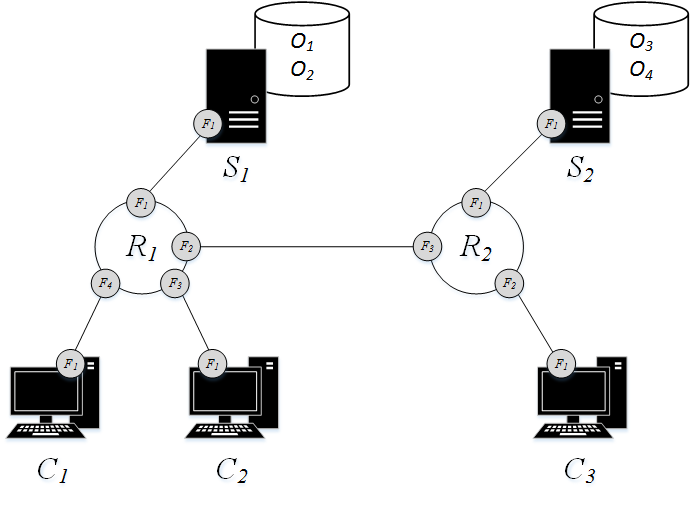
\includegraphics[width=0.30\textwidth] {figures/fib-topo.pdf}
        \label{fig:exp-results-time-cascade-random}
    }

    \cprotect\caption{Relative time spent at cache per content object. 
        Different cache algorithms --- LRU (a), MRU (b) and 
        random caching (c) --- cascade topology, $|L| = 5$, $|C| = 1$, 
        $|R| = 3$ and $|S| = 1$, $|P| = 25$, $\alpha = 1$.}
    \label{fig:exp-results-time-cascade}

\end{figure}

\begin{figure}[h!]
    \centering
    \subfigure[]{
        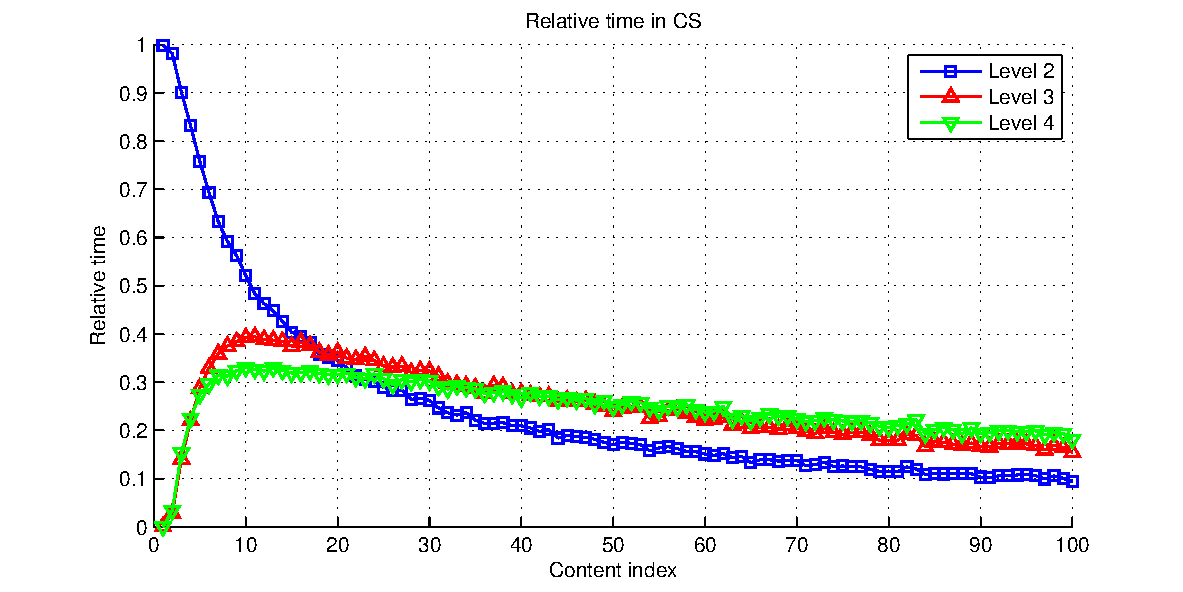
\includegraphics[width=0.40\textwidth] {figures/experiments/tree/LRU/25/6-4.pdf}
        %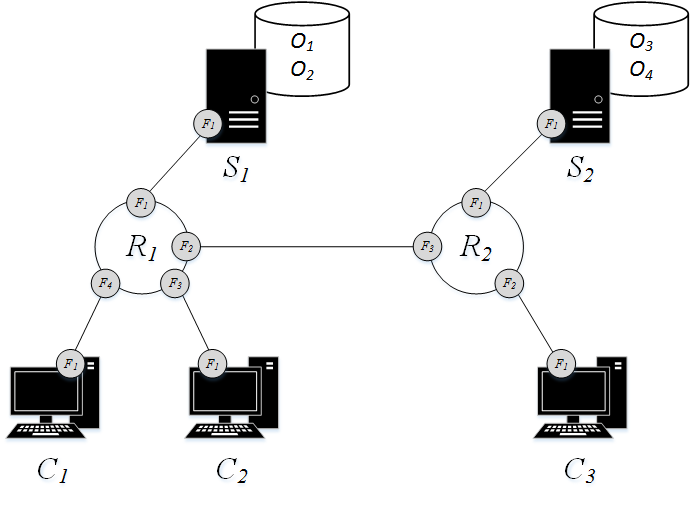
\includegraphics[width=0.30\textwidth] {figures/fib-topo.pdf}
        \label{fig:exp-results-time-tree-lru}
    }

    \subfigure[]{
        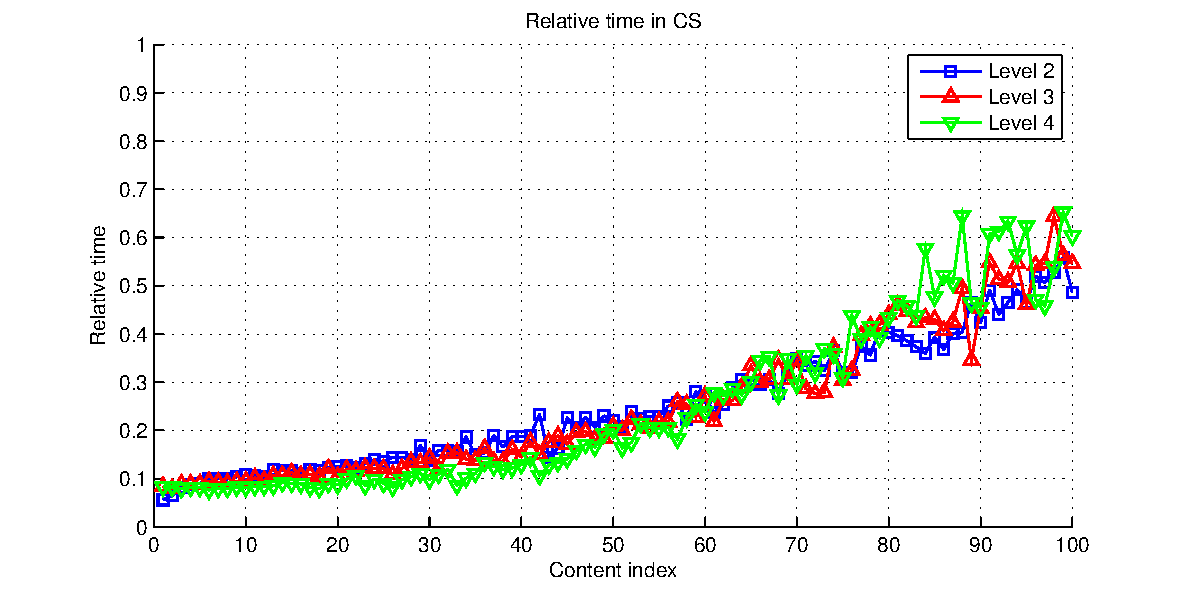
\includegraphics[width=0.40\textwidth] {figures/experiments/tree/MRU/25/6-4.pdf}
        %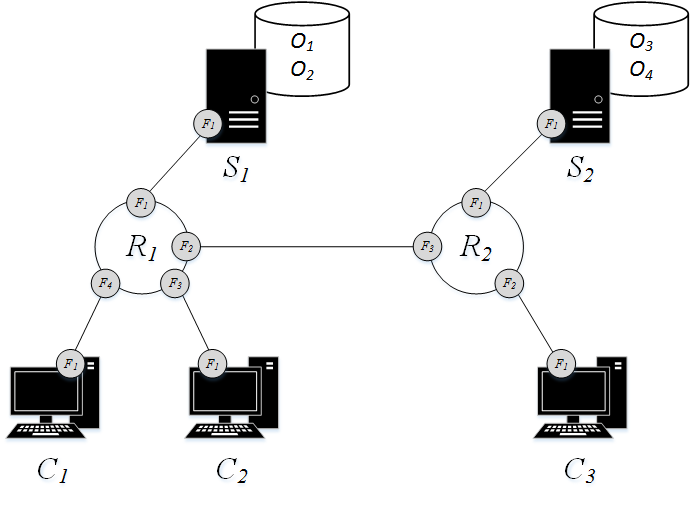
\includegraphics[width=0.30\textwidth] {figures/fib-topo.pdf}
        \label{fig:exp-results-time-tree-mru}
    }

    \subfigure[]{
        \includegraphics[width=0.40\textwidth] {figures/experiments/tree/RANDOM/25/6-4.pdf}
        %\includegraphics[width=0.30\textwidth] {figures/fib-topo.pdf}
        \label{fig:exp-results-time-tree-random}
    }

    \cprotect\caption{Relative time spent at cache per content object. 
        Different cache algorithms --- LRU (a), MRU (b) and 
        random caching (c) --- binary tree topology, $|L| = 5$, $|C| = 8$, 
        $|R| = 7$ and $|S| = 1$, $|P| = 25$, $\alpha = 1$.}
    \label{fig:exp-results-time-tree}

\end{figure}



%\section{Related Work}
\label{sec:rel-work}

The study of techniques for text classification presented here is mostly 
based on the work by McCallum et al.~\cite{McCallum98acomparison} and 
Nigam et al.~\cite{Nigam2000}, extensively covered 
in Section~\ref{sec:methodology}. Within the field of supervised 
learning, starting from the MNB model presented 
in~\cite{McCallum98acomparison}, Rennie et al.~\cite{Rennie03tacklingthe} 
propose a series of transforms, based on Information Retrieval 
techniques, which improve the performance of MNB, resulting 
in an enhanced method designated by Transformed Weight-normalized Complement 
Naive Bayes (TWCNB). In the semi-supervised scope, Mann et al.~\cite{Mann2007a} 
proposed a general approach to semi-supervised learning, but tested on 
text classification, designated by Expectation 
Regularization (XR)~\cite{Mann2007a}. XR is based on exponential-family 
parametric models, normally trained by MAP estimation. XR adds it with a second 
term, which attempts to minimize the difference between 
the predicted posteriors $P(Y|X)$ for unlabeled data and estimated pre-known 
values for $P(Y|X)$, obtained from empirical 
data or the labeled data. The method is tested against MNB and MNB + EM, being 
outperformed by the two in the Simulated\slash Real\slash Aviation\slash Auto 
(SRAA) text classification task, similar to 20 Newsgroups task.\vertbreak


\section{Discussion}
\label{sec:discussion}

Figures~\ref{fig:exp-results-topologies-cascade} and~\ref{fig:exp-results-topologies-tree} 
show a comparison of the quantity of Interest and Data packets received\slash sent 
per topology level, for both the cascade and binary tree topologies in 
Figure~\ref{fig:exp-setup-nettop}. Both topologies clearly show a significantly 
larger number of received Interest signals at level 2 (in fact, level 2 receives 
all the Interest signals generated by the clients at level 1), compared to 
a much smaller number of Interest signals relayed to the subsequent `upstream' 
levels. This is a result of two features of NDN: (1) the aggregation of Interest 
signals in PITs; and (2) cache hits in the CSs. Also note the 
difference in nearly one order of magnitude of the 
Interests forwarded `upstream' for both topologies, e.g. at level 2, $\sim2 \times 10^4$ Interest signals 
are forwarded for the cascade case, vs. $\sim1.5 \times 10^5$ in the binary 
tree topology case. This is obviously a consequence of the larger number of 
clients contained in the binary tree topology. The quantity of Interests forwarded 
`upstream' is generally larger in the case for the MRU cache algorithm, due to 
the smaller contribution of cache hits (e.g. as seen in 
Figure~\ref{fig:exp-results-cache-alg-cascade}). The differences between cache 
algorithms are accentuated in Data packet statistics: e.g. focusing on 
Figure~\ref{fig:exp-results-topologies-cascade}, while for LRU the quantity of 
Data packets sent by level 2 is practically equal to the number of received 
Interests, the same does not happen with MRU, with a difference of 
$4 \times 10^4$ to $\sim2.5 \times 10^4$. This is mostly due to the fact that 
MRU does not favor the most popular content, whose Interests have to be forwarded 
much further `upstream' to be satisfied, resulting in larger accumulations of 
pending Interests at lower levels. Another interesting phenomena is 
verified in Figure~\ref{fig:exp-results-topologies-tree-lru}, specifically 
regarding the binary tree topology: note how the quantity of Data packets 
received at level 1 far exceeds the generated Interest signals. This happens 
due to the sharing of the interfaces $F_{r,1}$ of the routers at level 1 per each pair of 
clients, and subsequent duplication of Data signals. Again, the difference is 
not exactly a 2:1 ratio due to the action of Interest signal aggregation at 
PITs.\shortvertbreak

Figures~\ref{fig:exp-results-cache-alg-cascade} and~\ref{fig:exp-results-cache-alg-tree} 
show the cache hit\slash miss rates for the different topologies and all considered 
caching algorithms. One can notice a similarity in the trends of the LRU and Random caching 
algorithms, both favoring the most popular content, i.e. objects $O_o$ with 
$1 \le o \le 30$. For both topology types and LRU policy, level 2 (the first level after the 
`layer' of clients) exhibits significantly larger cache hit rates for the most 
popular content than on subsequent `upstream' levels. This indicates 
that CSs at level 2 become mostly occupied by popular content objects, hence explaining 
the results previously analyzed in Figures~\ref{fig:exp-results-topologies-cascade} 
and~\ref{fig:exp-results-topologies-tree}. Such differences between levels are 
only verified with the LRU algorithm, being mitigated with Random caching. This 
behavior can be explained by the nature of the 
two algorithms: upon the arrival of new Data packets at a full CS, the LRU 
caching policy chooses infrequently requested content ($O_o$ with $o > 30$) for 
eviction, while the Random caching algorithm does not discriminate 
particular content indexes, choosing eviction candidates according to an 
uniform distribution. Therefore, while with LRU `stockpiles' objects 
$1 \le o \le 30$ at the first layer of caches (i.e. level 2), Random caching 
distributes them over all levels.\shortvertbreak

The 
MRU algorithm --- see Figures~\ref{fig:exp-results-cache-alg-cascade-mru} 
and~\ref{fig:exp-results-cache-alg-tree-mru} --- follows an opposite trend, 
favoring the less popular content and `flattening' the overall hit rates (at lower 
values). In fact, these results somehow show the unsuitability of the MRU cache 
algorithm for the model of Interest signal generation we consider here, i.e. with 
independent inter-arrival times. The MRU algorithm is mostly indicated for 
situations in which the inter-arrival times of events are not independent between 
each other, e.g. in cases where the occurrence of some event $e$ at some point 
in time indicates that the same event is unlikely to occur in the near future. On the 
other hand, the LRU algorithm, designed to favor events which are likely to be occur 
in `bursts' and concentrated in specific time periods, favors popular content (whose Interest 
generation occurs more often and therefore exhibiting smaller intervals between occurrences), 
despite our usage of independent inter-arrival times.\shortvertbreak

The differences between 
Figures~\ref{fig:exp-results-cache-alg-cascade-lru} 
and~\ref{fig:exp-results-cache-alg-tree-lru} seem to indicate a larger `caching 
capacity' for the binary tree topology, as it presents overall larger hit rate 
values across all content objects. This is not surprising, due to the 
larger number of routers (and hence cache capacity) per level.\shortvertbreak

Figures~\ref{fig:exp-results-latency-cascade} and~\ref{fig:exp-results-latency-tree} show 
the ratio of received Interests to original requests, per content object 
and network level (including server(s) $S$), for both topology types considered in the 
experiments. These charts is provide an idea of the `latency' a client can expect for 
the satisfaction of an Interest for some content object, in the sense that it shows how far (i.e. to 
which level) are Interests forwarded `upstream'. Overall, and for both topologies, 
the following aspects can be highlighted: 

\begin{itemize}
    \item All original Interest requests are 
        received by level 2 (the first layer of routers after the clients), as expected, since 
        we are not considering any packet losses between interconnected topology elements;
    \item For the LRU and Random cache algorithms, the ratio is greatly reduced for 
        the most popular content objects, with values $\sim0$ for the LRU algorithm, 
        indicating that these content instances are mostly cached and served at 
        lower levels of the topologies, and therefore accessed with lower latencies;
    \item For both LRU and Random algorithms, the ratio values increase with the index of 
        content objects, i.e. with the reduction of their popularity, indicating that 
        Interests for less popular content tend to cross more topology levels and 
        are therefore accessed with larger latencies (e.g. in the case of $O_{100}$ 
        the ratio value of level 5 --- of the server $S$ --- is contained in the 
        interval $[0.5, 0.8]$, meaning 
        that more that $50\%$ of the Interest signals for $O_{100}$ need to actually 
        reach $S$ to be satisfied). As the more popular content `hijacks' CS space 
        at lower topology levels, being constantly refreshed by frequent cache 
        hits, Interest signals for unpopular content must reach CSs at higher levels;
    \item The ratio values for a given content object tend to decrease with the topology 
        levels, both as a result of (1) aggregation of pending Interests at PITs and 
        (2) cache hits.
\end{itemize}\shortvertbreak

One can note a difference between Figures~\ref{fig:exp-results-latency-cascade-lru} 
and~\ref{fig:exp-results-latency-tree-lru}, both pertaining to the LRU cache 
algorithm, but under different topologies: in the former, the differences in 
ratio values between levels are nearly absent, while in the latter, a clear difference 
can be identified. The same pattern is evident in 
Figures~\ref{fig:exp-results-topologies-cascade-lru} and~\ref{fig:exp-results-topologies-tree-lru}. 
This behavior can be explained by the larger `caching capacity' of the binary 
tree topology.\shortvertbreak

The results for the MRU cache algorithm (Figures~\ref{fig:exp-results-latency-cascade-mru} 
and~\ref{fig:exp-results-latency-tree-mru}) show a trend for benefiting less 
popular content. The ratio values for the 
most popular content ($O_1$ to $O_2$) are low due to the number of Interests aggregated 
at PITs at level 2, and not to a high cache hit rate, as previously identified in Figures~\ref{fig:exp-results-cache-alg-cascade-mru} 
and~\ref{fig:exp-results-cache-alg-tree-mru}. As MRU favors the caching of less popular 
content, the ratio values decrease with the index of content objects. Also note how the 
results for the cascade topology are more `unstable' that those of the binary 
tree case: this is due to difference in nearly one order of magnitude of the 
Interests forwarded `upstream', e.g. at level 2, $\sim2 \times 10^4$ Interest signals 
are forwarded for the cascade case, vs. $\sim1.5 \times 10^5$ in the binary 
tree topology case.\shortvertbreak

Finally, in Figures~\ref{fig:exp-results-time-cascade} 
and~\ref{fig:exp-results-time-tree}, we present the results for our last 
metric, the relative time spent at CSs, per content object and topology level. 
Here the differences between cache algorithms are much more evident than those 
between topologies. In the case of LRU, Figures~\ref{fig:exp-results-time-cascade-lru} 
and~\ref{fig:exp-results-time-tree-lru}, one can verify that content objects $O_1$ 
to $O_{10}$ are located in caches for $> 50\%$ of the simulation rounds in 
level 2, and nearly absent in levels 3 and 4. This seems to accentuate the 
idea that the exchanges of popular content are concentrated between levels 1 and 2. 
Objects $O_o$ with $o > 10$ spend more time cached at the subsequent 
levels, with relative times in the interval $[0.4, 0.1]$. Note how the binary tree's 
larger `caching capacity' rises the relative caching time of objects 
$O_o$ with $o > 10$, as well as a reduction for $1 \le o \le 10$ in levels 3 
and 4. The results for the Random cache algorithm, Figures~\ref{fig:exp-results-time-cascade-random} 
and~\ref{fig:exp-results-time-tree-random}, follow a similar 
trend to that of LRU, nevertheless with larger relative caching times for content 
objects $O_1$ to $O_{10}$ on levels 3 and 4, and a subsequent reduction for 
level 2. Regarding the MRU caching policy, the benefit of less popular content 
is also verified in Figures~\ref{fig:exp-results-time-cascade-mru} 
and~\ref{fig:exp-results-time-tree-mru}, as one notes the increase in relative 
caching time for larger content indexes, without major differences between levels. 
Furthermore, the results for the binary tree topology seem more `stable', once again 
probably due to the due to difference in nearly one order of magnitude of the 
Interests forwarded `upstream'.



\section{Conclusions}

In this work we study the field of semi-supervised learning, applied to the 
field of text classification. We closely follow the work in~\cite{McCallum98acomparison,Nigam2000}, reporting out 
understanding of the presented models.\vertbreak

We follow the methods presented by Nigam et al.~\cite{Nigam2000} to implement our 
versions of the MNB and MNB + EM (including EM-$\lambda$) approaches. We 
take the well-known 20 Newsgroups dataset~\cite{Lang95}, particularly 
a version designated by \verb+20news-bydate+, to evaluate the studied 
semi-supervised models in the context of a real-world dataset. The 
\verb+20news-bydate+ dataset is manipulated using the Rainbow tools --- developed 
by the authors of the base literature reviewed in this paper --- in order to 
pre-process it according to commonly used procedures and divide it 
into training and test partitions, also creating unlabeled samples for the 
semi-supervised setting.\vertbreak

Our version of MNB is compared with Rainbow's, producing lower accuracy values 
for small amounts of labeled data, approaching Rainbow's accuracy rates for 
higher amounts of labeled data ($|A^\ell| > 5000$). Due to problems with our 
implementation of MNB + EM, making its results unsuitable for comparison, we 
use Rainbow's implementation of MNB + EM and EM-$\lambda$ over the 
\verb+20news-bydate+ dataset to experimentally validate the previously studied 
semi-supervised methods. We verify that, on average MNB + EM performs better 
than MNB for $|A^\ell| < 100$, with $11220 \le |A^u| \le 11240$. We also verify that, 
despite its large variations, for at least one of the test runs performed 
for every $|A^\ell|$, MNB + EM surpasses MNB. Regarding EM-$\lambda$, while 
smaller weights for unlabeled data seem to favor accuracy for larger 
$|A^\ell|$, the best results are always obtained for $\lambda = 1$. For 
$|A^\ell| \ge 1000$, the results seem intuitive, as the accuracy approaches 
that of MNB for smaller values of $\lambda$ (i.e. smaller weights given to 
the unlabeled data).


\bibliographystyle{unsrt}
\bibliography{mtsp}

\end{document}
